\documentclass[10pt, a4j, dvipdfmx]{jarticle}
\usepackage{titlesec}
\usepackage[dvipdfmx]{graphicx}
\usepackage[dvipdfmx]{color}
\usepackage{float}
\usepackage{wrapfig}
\usepackage{subfigure}
\usepackage{caption}

\makeatletter
\newcommand{\figcaption}[1]{\def\@captype{figure}\caption{#1}}
\newcommand{\tblcaption}[1]{\def\@captype{table}\caption{#1}}
\makeatother

\title{ディジタル回路III}
\author{4年 電子システム工学科 40番  山地 駿徹}

\begin{document}
\section{目的}
演算増幅器を使用した基本回路や演算回路を制作することにより,演算増幅の基本動作の理解を深める.


\section{原理}
演算増幅器は,2個の入力端子と1個の出力端子を持つ増幅器で-側の入力端子に入力信号を加えると同相の増幅出力が得られる.
また2個の入力端子に大きさ,位相の等しい信号を加えると出力は零となる.

一般に演算増幅器は,帰還回路を組み合わせることにより,全体の特性が帰還回路の特性だけで決まるような条件で,動作させることを目的とした高利得増幅器で,原則として低域遮断周波数が零ヘルツの直流電圧増幅器である.


\section{演算増幅器の特徴}
演算増幅器の主とした特徴は下記の五項目である.
\begin{enumerate}
    \renewcommand{\labelenumi}{(\arabic{enumi})}
    \item 差動入力素子である.
    \item 増幅度が非常に大きい.
    \item 入力インピーダンスが非常に大きい.                                                                                                                                                                                                                                                     
    \item 出力インピーダンスが小さい.
    \item 周波数帯域幅が非常に広い.
    \item 雑音が非常に小さい.
\end{enumerate}

\newpage
\section{演算増幅回路の基本的動作}
\renewcommand{\thesubsection}{[\Alph{subsection}]}
\subsection{反転増幅回路の動作}
\begin{wrapfigure}{r}{55mm}
    \vspace*{-\intextsep}
    \begin{center}
     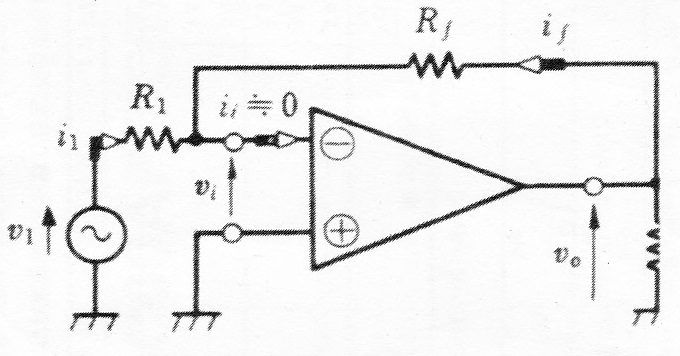
\includegraphics[width=50mm]{text/fig-1.jpg}
     \caption{反転増幅回路}
    \end{center}
\end{wrapfigure}
図1の演算増幅回路において,演算増幅器が向き感じの電圧増幅度$A_v = V_o / V_i$となり,負帰還時の電圧増幅度$A_{vf} = V_o / V_1$である.
キルヒホッフの法則から回路に流れる電流は(1)となる.
\begin{equation}
    i_1 + i_f = i_i
\end{equation}

演算増幅器の特徴から,入力インピーダンス$Z_i$は非常に大きいから演算増幅器への入力電流$i_i$はほとんど流れない.
従って,$i_i \approx -i_i$となる.

図1の反転増幅回路にキルヒホッフの法則を適用すると(2),(3)式を得る.
\begin{eqnarray}
    V_o - V_i & = & -r_f i_i \\
    V_o - V_1 & = &  -R_f i_i - R_1 i_1
\end{eqnarray}

また,演算増幅器の電圧増幅度$A_v$は非常に大きく$V_o \gg V_i$であるから,(2)式は(4)式で表される.
\begin{equation}
    V_o \approx -R_f i_1
\end{equation}

更に(3), (4)式から(5)式を得る.
\begin{equation}
    V_1 \approx R_1 i_1
\end{equation}
演算増幅器の入力端は,イマジナリショートしていると考えられるから,負帰還時の電圧増幅度$A_{vf}$を(4),(5)式から求めると(6)式となる.
\begin{equation}
    A_{vf} = V_o / V_1 \approx -R_f / R_1
\end{equation}
(6)式の$A_{vf}$は抵抗$R_f$と$R_1$によって決定される.
またこの式の-符号は,入力と出力が逆位相であることを示している.

\emph{回路制作では$R_1$を$1[k\Omega]$, $R_f$を$10[k\Omega]$とする.}


\subsection{非反転増幅回路の動作}
\begin{wrapfigure}{r}{55mm}
    \vspace*{-\intextsep}
    \begin{center}
     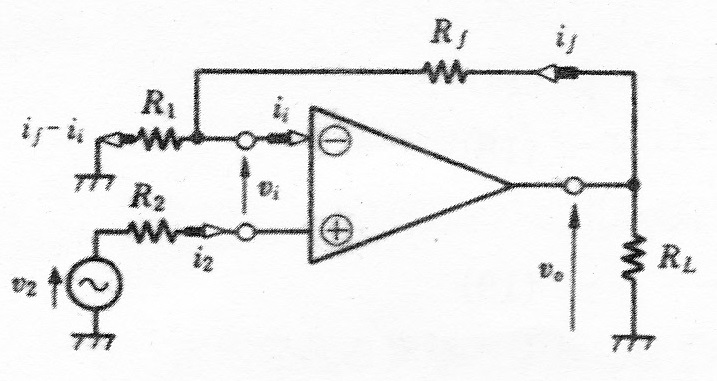
\includegraphics[width=50mm]{text/fig-2.jpg}
     \caption{非反転増幅回路}
    \end{center}
\end{wrapfigure}
図2において,演算増幅回路にキルヒホッフの法則を適用すると(7), (8)式を得る.
\begin{eqnarray}
    V_2 - V_1 & = & R_2 i_2 + R_1 (i_f - i_i) \\
    V_o & = & R_f i_f + R_1 (i_f i_i)
\end{eqnarray}
この(7),(8)式にイマジナリショートの制約を適用すると(9),(10)式を得る.
\begin{eqnarray}
    V_2 & \approx & R_1 i_f \\
    V_o & \approx & (R_f + R_1) i_f
\end{eqnarray}
これより,非反転増幅回路の電源電圧$A_{vf}$は(11)式となる.
\begin{equation}
    A_{vf} = V_o / V_2 \approx (R_1 + R_f) / R_1 = 1 + R_f / R_1
\end{equation}
(11)四季は入力と出力が同位相であることを示している.

\emph{回路制作では$R_1$を$1[k\Omega]$,$R_f$を$10[k\Omega]$とする.}


\subsection{加算増幅回路の動作}
\begin{wrapfigure}{r}{55mm}
    \vspace*{-\intextsep}
    \begin{center}
     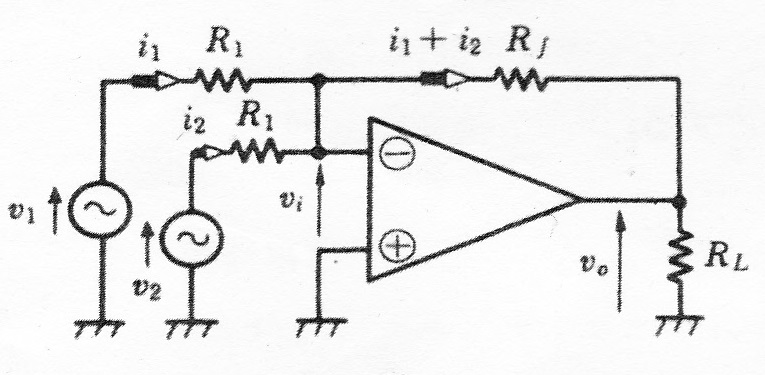
\includegraphics[width=50mm]{text/fig-3.jpg}
     \caption{加算回路}
    \end{center}
\end{wrapfigure}
図3において,演算増幅器の入力端にイマジナリショートの制約を適用して回路の$i_i$,$i_2$を求めると(12),(13)式を得る.
\begin{eqnarray}
    i_1 & \approx & V_1 / R_1 \\
    i_2 & \approx & V_2 / R_1
\end{eqnarray}
また,出力電圧$V_o$は(14)式となる.
\begin{equation}
    V_o = -R_f (i_1 + i_2)
\end{equation}
さらに,(12),(13)及び(14)式より出力電圧$V_o$を求めると(15)式を得る.
\begin{equation}
    V_o = -R_f (V_1 / R_1 + V_2 / R_1) = -R_f / R_1 (V_1 + V_2)
\end{equation}
(15)式の$R_1 = R_f$とおくと出力電圧$V_o$は(16)式となる.
\begin{equation}
    V_o = -(V_1 + V_2)
\end{equation}
従って,入力電圧が加算された出力電圧となる.

\emph{回路制作では$R_1$を$1[k\Omega]$,$R_f$を$10[k\Omega]$とする.}


\subsection{減算増幅回路の動作}
\begin{wrapfigure}{r}{55mm}
    \vspace*{-\intextsep}
    \begin{center}
     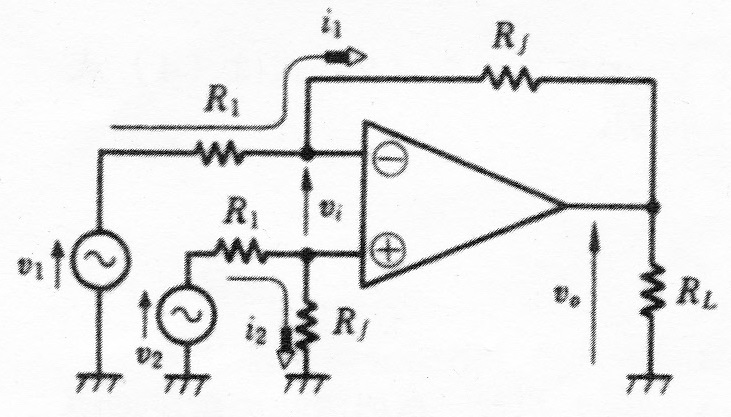
\includegraphics[width=50mm]{text/fig-4.jpg}
     \caption{減算回路}
    \end{center}
\end{wrapfigure}
図4において,演算増幅器の入力端にイマジナリショートの制約を適用して回路の$i_2$,$V_1$を求めると(17), (18)式を得る.
\begin{eqnarray}
    i_2 & \approx & V_2 / (R_1 + R_f) \\
    V_1 & \approx & R_1 i_1 + R_f i_2
\end{eqnarray}
また,出力電圧$V_o$は(19)式となる.
\begin{equation}
    V_o \approx -R_f i_1 + R_f i_2
\end{equation}
(17),(18)及び(19)式より出力電圧を求めると(20)式を得る.
\begin{equation}
    V_o = R_f / R_1 (V_2 - V_1)
\end{equation}
(20)式の$R_1 = R_f$とおくと,出力電圧$V_o$は(21)式となる.
\begin{equation}
    V_o = V_2 - V_1
\end{equation}
従って,入力電圧が減算された出力電圧となる.

\emph{回路制作では$R_1$を$1[k\Omega]$,$R_f$を$10[k\Omega]$とする.}


\newpage
\section{基本回路の実験方法}
\renewcommand{\thesubsection}{\arabic{section}.\arabic{subsection}}
\subsection{[反転増幅回路の特性測定]}
\renewcommand{\labelenumi}{(\arabic{enumi})}
\begin{enumerate}
    \item 図1のように結線し,発振器の周波数を$1[kHz]$にする.
    \item 反転増幅回路に入力電圧$V_1$を可変して入力し,その時の出力電圧$V_o$を測定する.
    \item 反転増幅回路の入力電圧$V_1$に対する出力電圧$V_o$をグラフ化し,伝達特性として表す.
    \item 歪み波形の観測及び波形のスケッチはオシロスコープを使用する.
\end{enumerate}
\subsection{[非反転増幅回路の特性測定]}
\begin{enumerate}
    \item 図2のように結線し,発振器の周波数を$1[kHz]$にする.
    \item 非反転増幅回路に入力電圧$v_1$を可変して入力し,その時の出力電圧$V_o$をデジタルボルトメーターで測定する.但し,出力電圧が飽和した範囲については,オシロスコープを用いて測定する.
    \item 非反転増幅回路の入力電圧$V_1$に対する出力電圧$V_o$をグラフ化し,伝達特性として表す.
    \item 歪み波形の観測及び波形のスケッチはオシロスコープを使用する.
\end{enumerate}
\subsection{[加算回路の特性測定]}
\begin{enumerate}
    \item 図2のように結線し,発振器の周波数を$1[kHz]$にする.
    \item 2入力加算回路の一方の入力電圧$V_2$を固定し,他方の入力電圧$V_1$を可変して,その時の出力電圧$V_o$を測定する.
    \item 2入力加算回路の入力電圧$V_1$~$V_2$に対する出力電圧$V_o$をグラフ化する.(各自で考えてグラフ化する.)
    % \item 歪み波形の観測及び波形のスケッチはオシロスコープを使用する.
\end{enumerate}
\subsection{[減算増幅回路の特性測定]}
\begin{enumerate}
    \item 図2のように結線し,発振器の周波数を$1[kHz]$にする.
    \item 2入力加算回路の一方の入力電圧$V_2$を固定し,他方の入力電圧$V_1$を可変して,その時の出力電圧$V_o$を測定する.
    \item 2入力加算回路の入力電圧$V_1$~$V_2$に対する出力電圧$V_o$をグラフ化する.(各自で考えてグラフ化する.)
    % \item 歪み波形の観測及び波形のスケッチはオシロスコープを使用する.
\end{enumerate}


\newpage
\section{応用回路の実験方法及び結果の処理}
\begin{enumerate}
    \item 演算増幅器を使用した積分回路を構成し,発振器から$1[kHz]$の矩形波を入力し,出力波形を観察して波形を記録せよ.回路素子に接続する抵抗を$10[k\Omega]$程度に固定して測定する.
    \item 次に回路素子のコンデンサを取り替えて,時定数を変化させ(1)の測定を行い,演算増幅器を使用した積分回路の時定数に対する応答特性を求める.
\end{enumerate}


\newpage
\section{結果の処理}
\subsection{[反転増幅回路の特性測定結果の処理]}
5.1に示した実験について,以下の表\ref{tbl:7-1-1}に測定結果を,図\ref{fig:7-1-1}に測定結果をもとに作成した伝達特性のグラフを示す.
\begin{figure}[H]
	\begin{tabular}{cc}
		\begin{minipage}{0.33\hsize}
			\normalsize
			\tblcaption{測定値}
			\label{tbl:7-1-1}
			\centering
			\small
			\begin{tabular}{|r|r|}\hline
                入力電圧 Vi  [V] & 出力電圧 Vo [V] \\\hline
                0.01 & 0.09 \\\hline
                0.02 & 0.20 \\\hline
                0.03 & 0.29 \\\hline
                0.04 & 0.40 \\\hline
                0.05 & 0.49 \\\hline
                0.06 & 0.58 \\\hline
                0.07 & 0.68 \\\hline
                0.08 & 0.78 \\\hline
                0.09 & 0.88 \\\hline
                0.10 & 0.98 \\\hline
                0.50 & 4.92 \\\hline
                1.00 & 9.12 \\\hline
                1.50 & 10.30 \\\hline
                2.00 & 10.90 \\\hline
                2.50 & 11.30 \\\hline
                3.00 & 11.60 \\\hline
                4.00 & 11.90 \\\hline
                5.00 & 12.00 \\\hline
                8.12 & 12.20 \\\hline
                \end{tabular}
			\normalsize
		\end{minipage}
		\begin{minipage}{0.66\hsize}
			\centering
			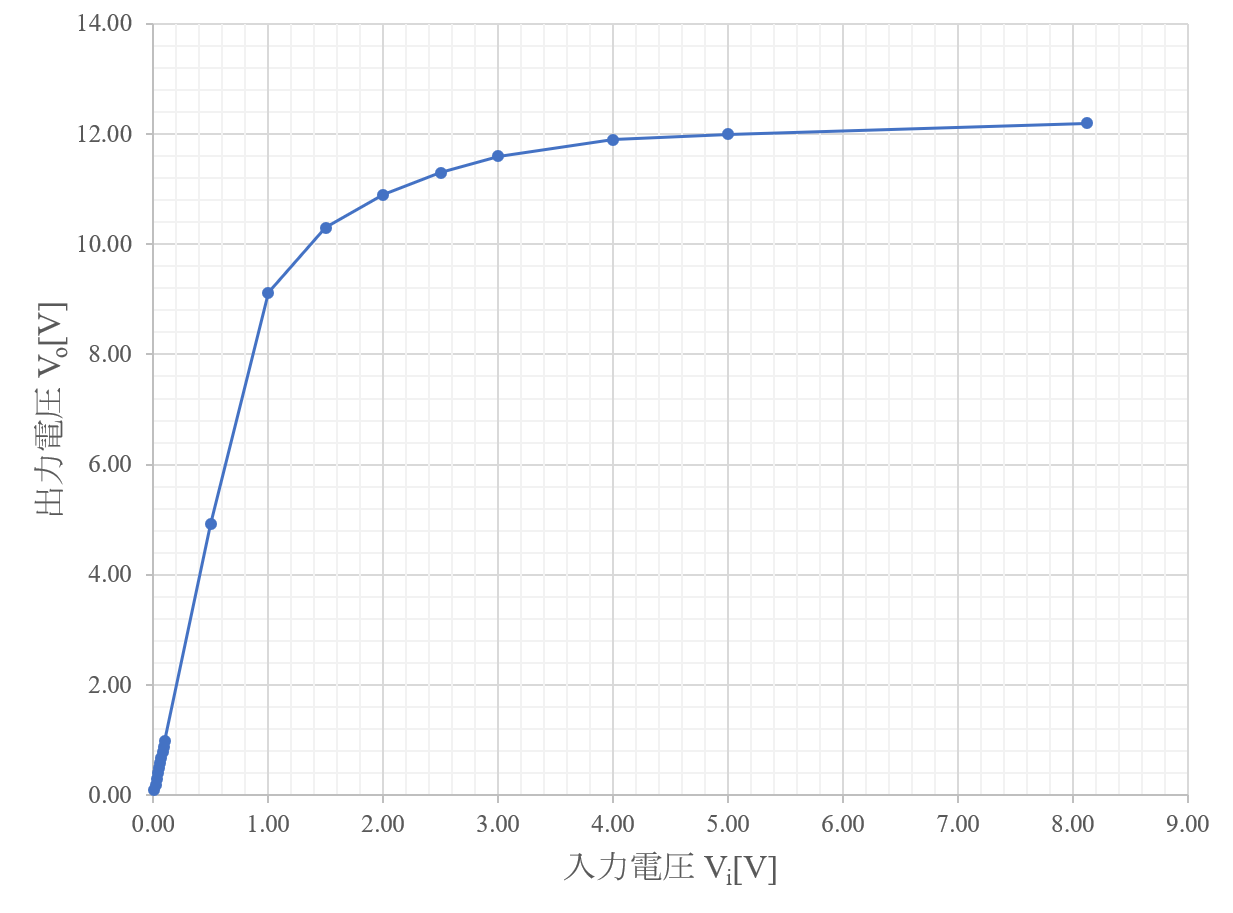
\includegraphics[width = 0.9\hsize]{experiment/7-1-1.png}
			\figcaption{制作した反転増幅回路の伝達特性}
			\label{fig:7-1-1}
		\end{minipage}
	\end{tabular}
\end{figure}
    また.以下の図\ref{fig:7-1-2}~\ref{fig:7-1-4}にデジタルオシロスコープを用いて測定した歪み波形を示す.
\begin{figure}[H]
    \centering
    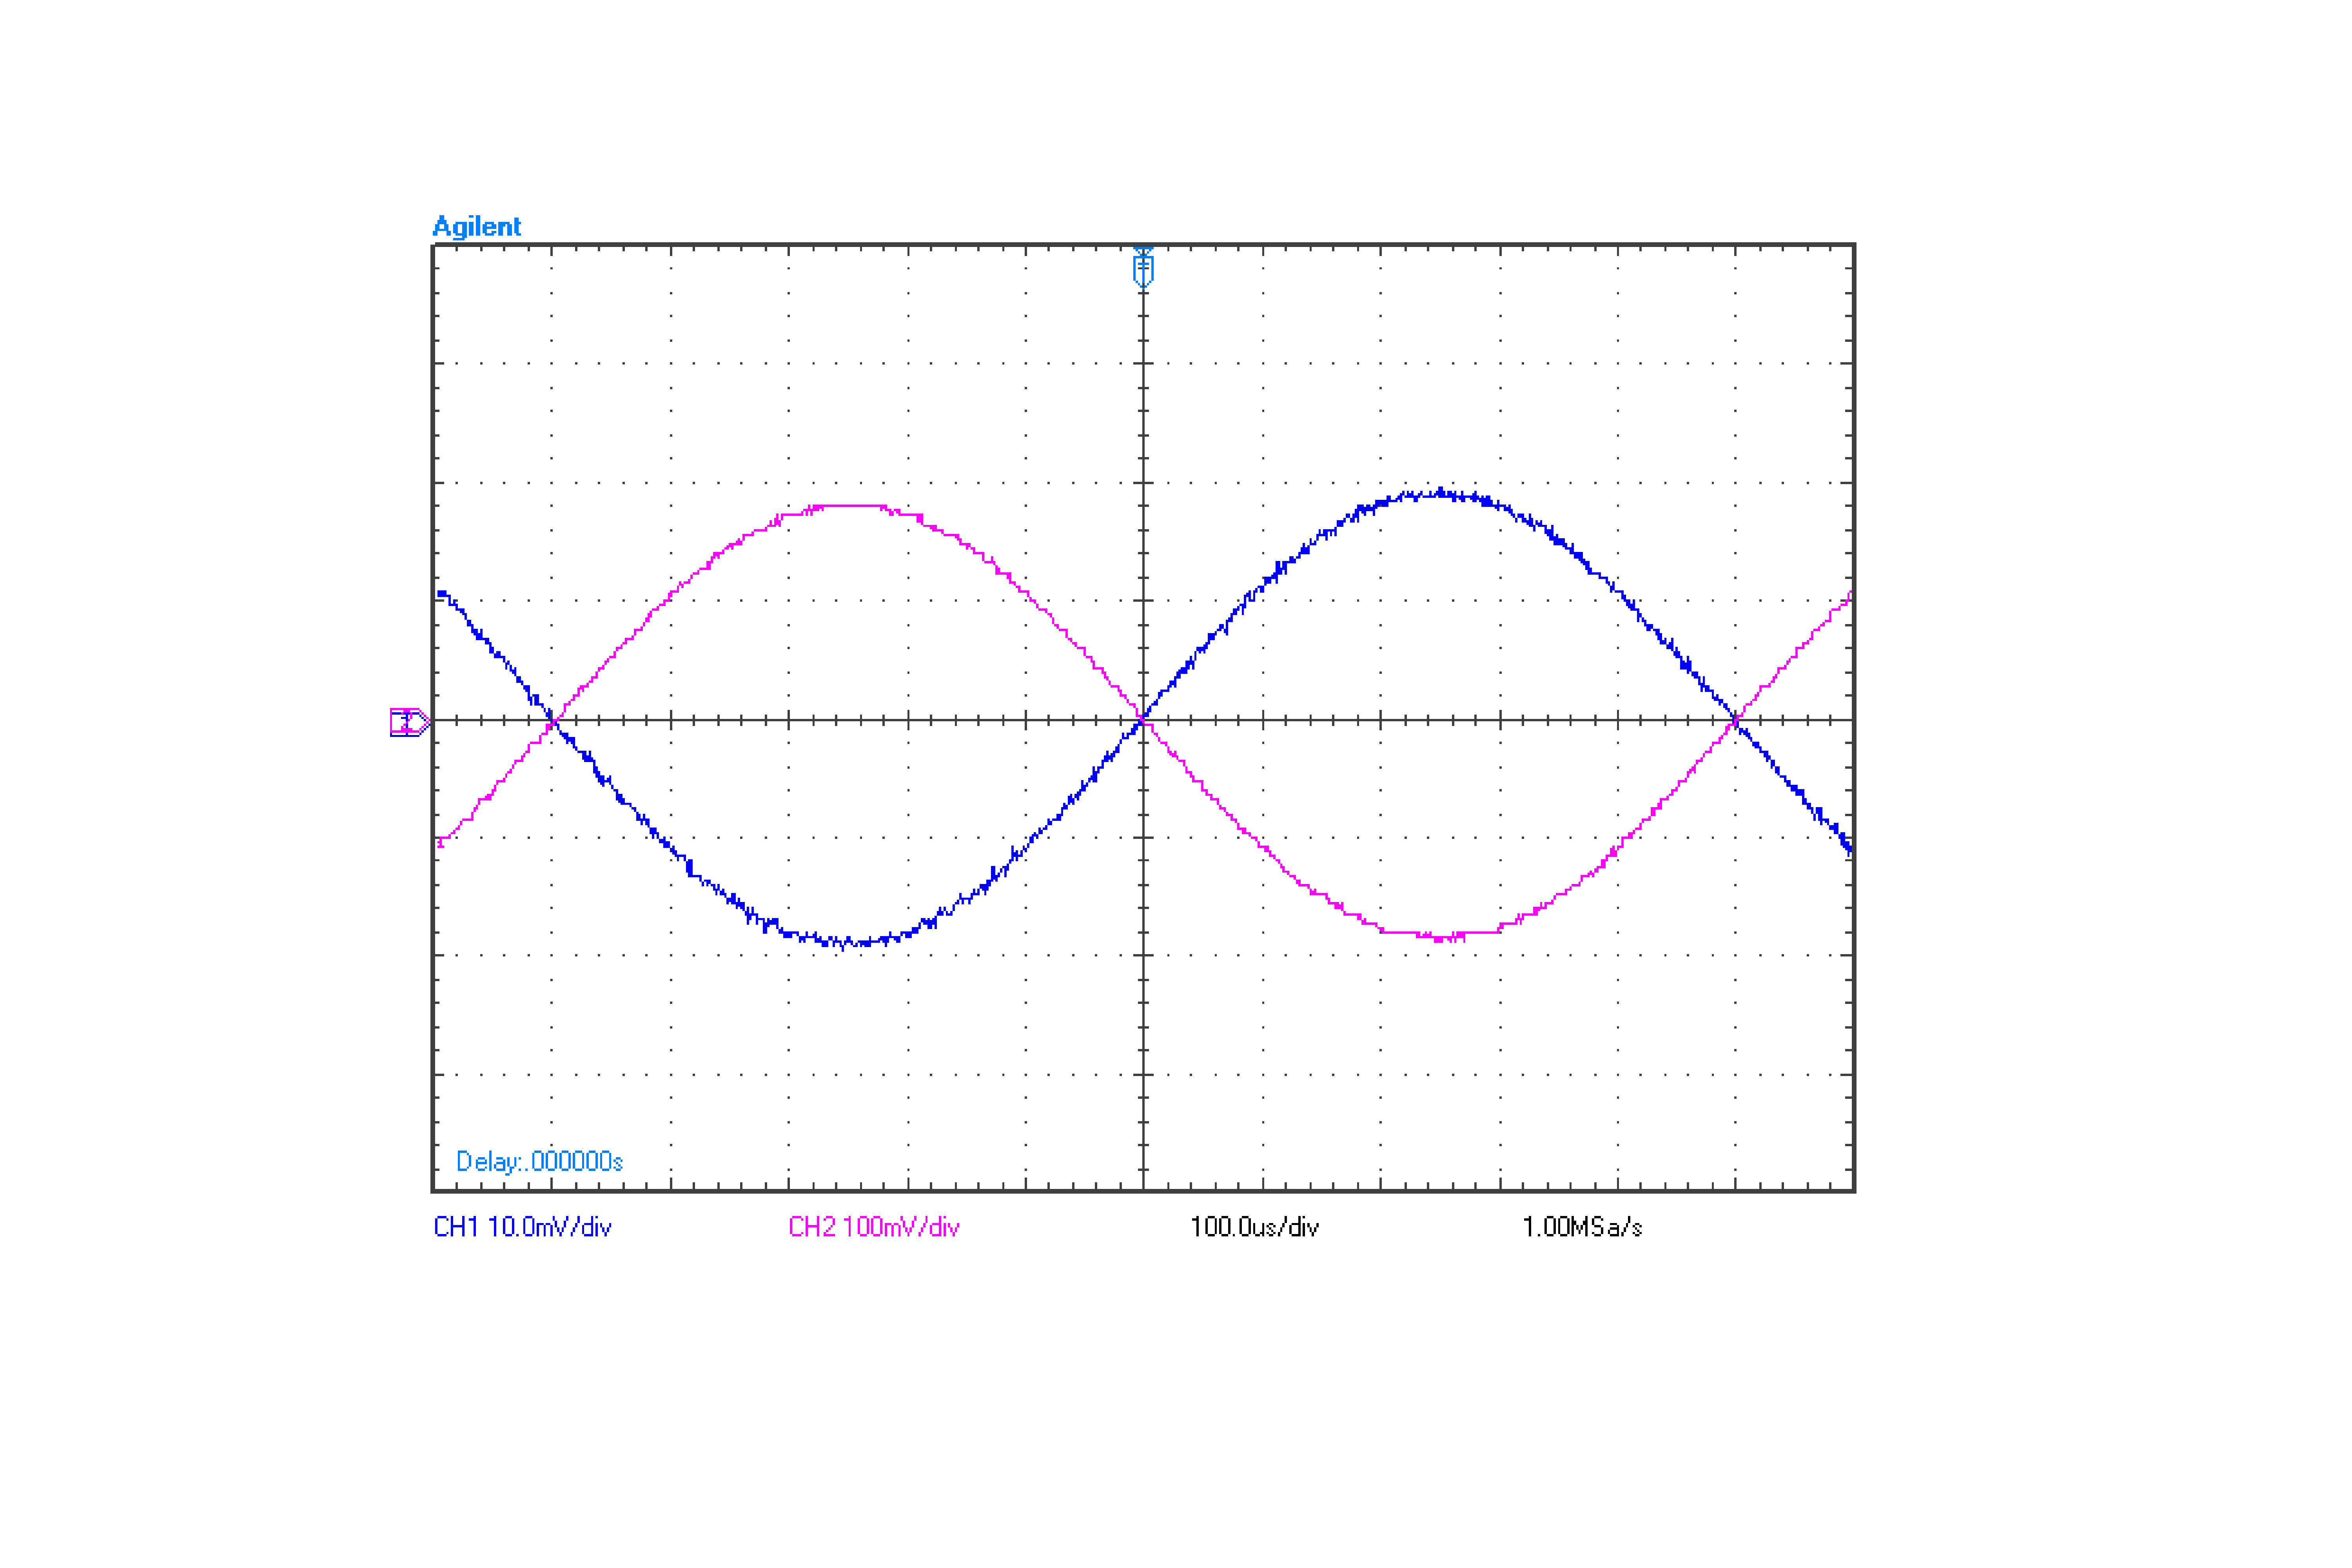
\includegraphics[height=70mm]{Result/Reverse/reverse-Hannten(input_10mV_output_95mV).png}
    \figcaption{歪みのない波形}
    \label{fig:7-1-2}
\end{figure}
\begin{figure}[H]
    \centering
    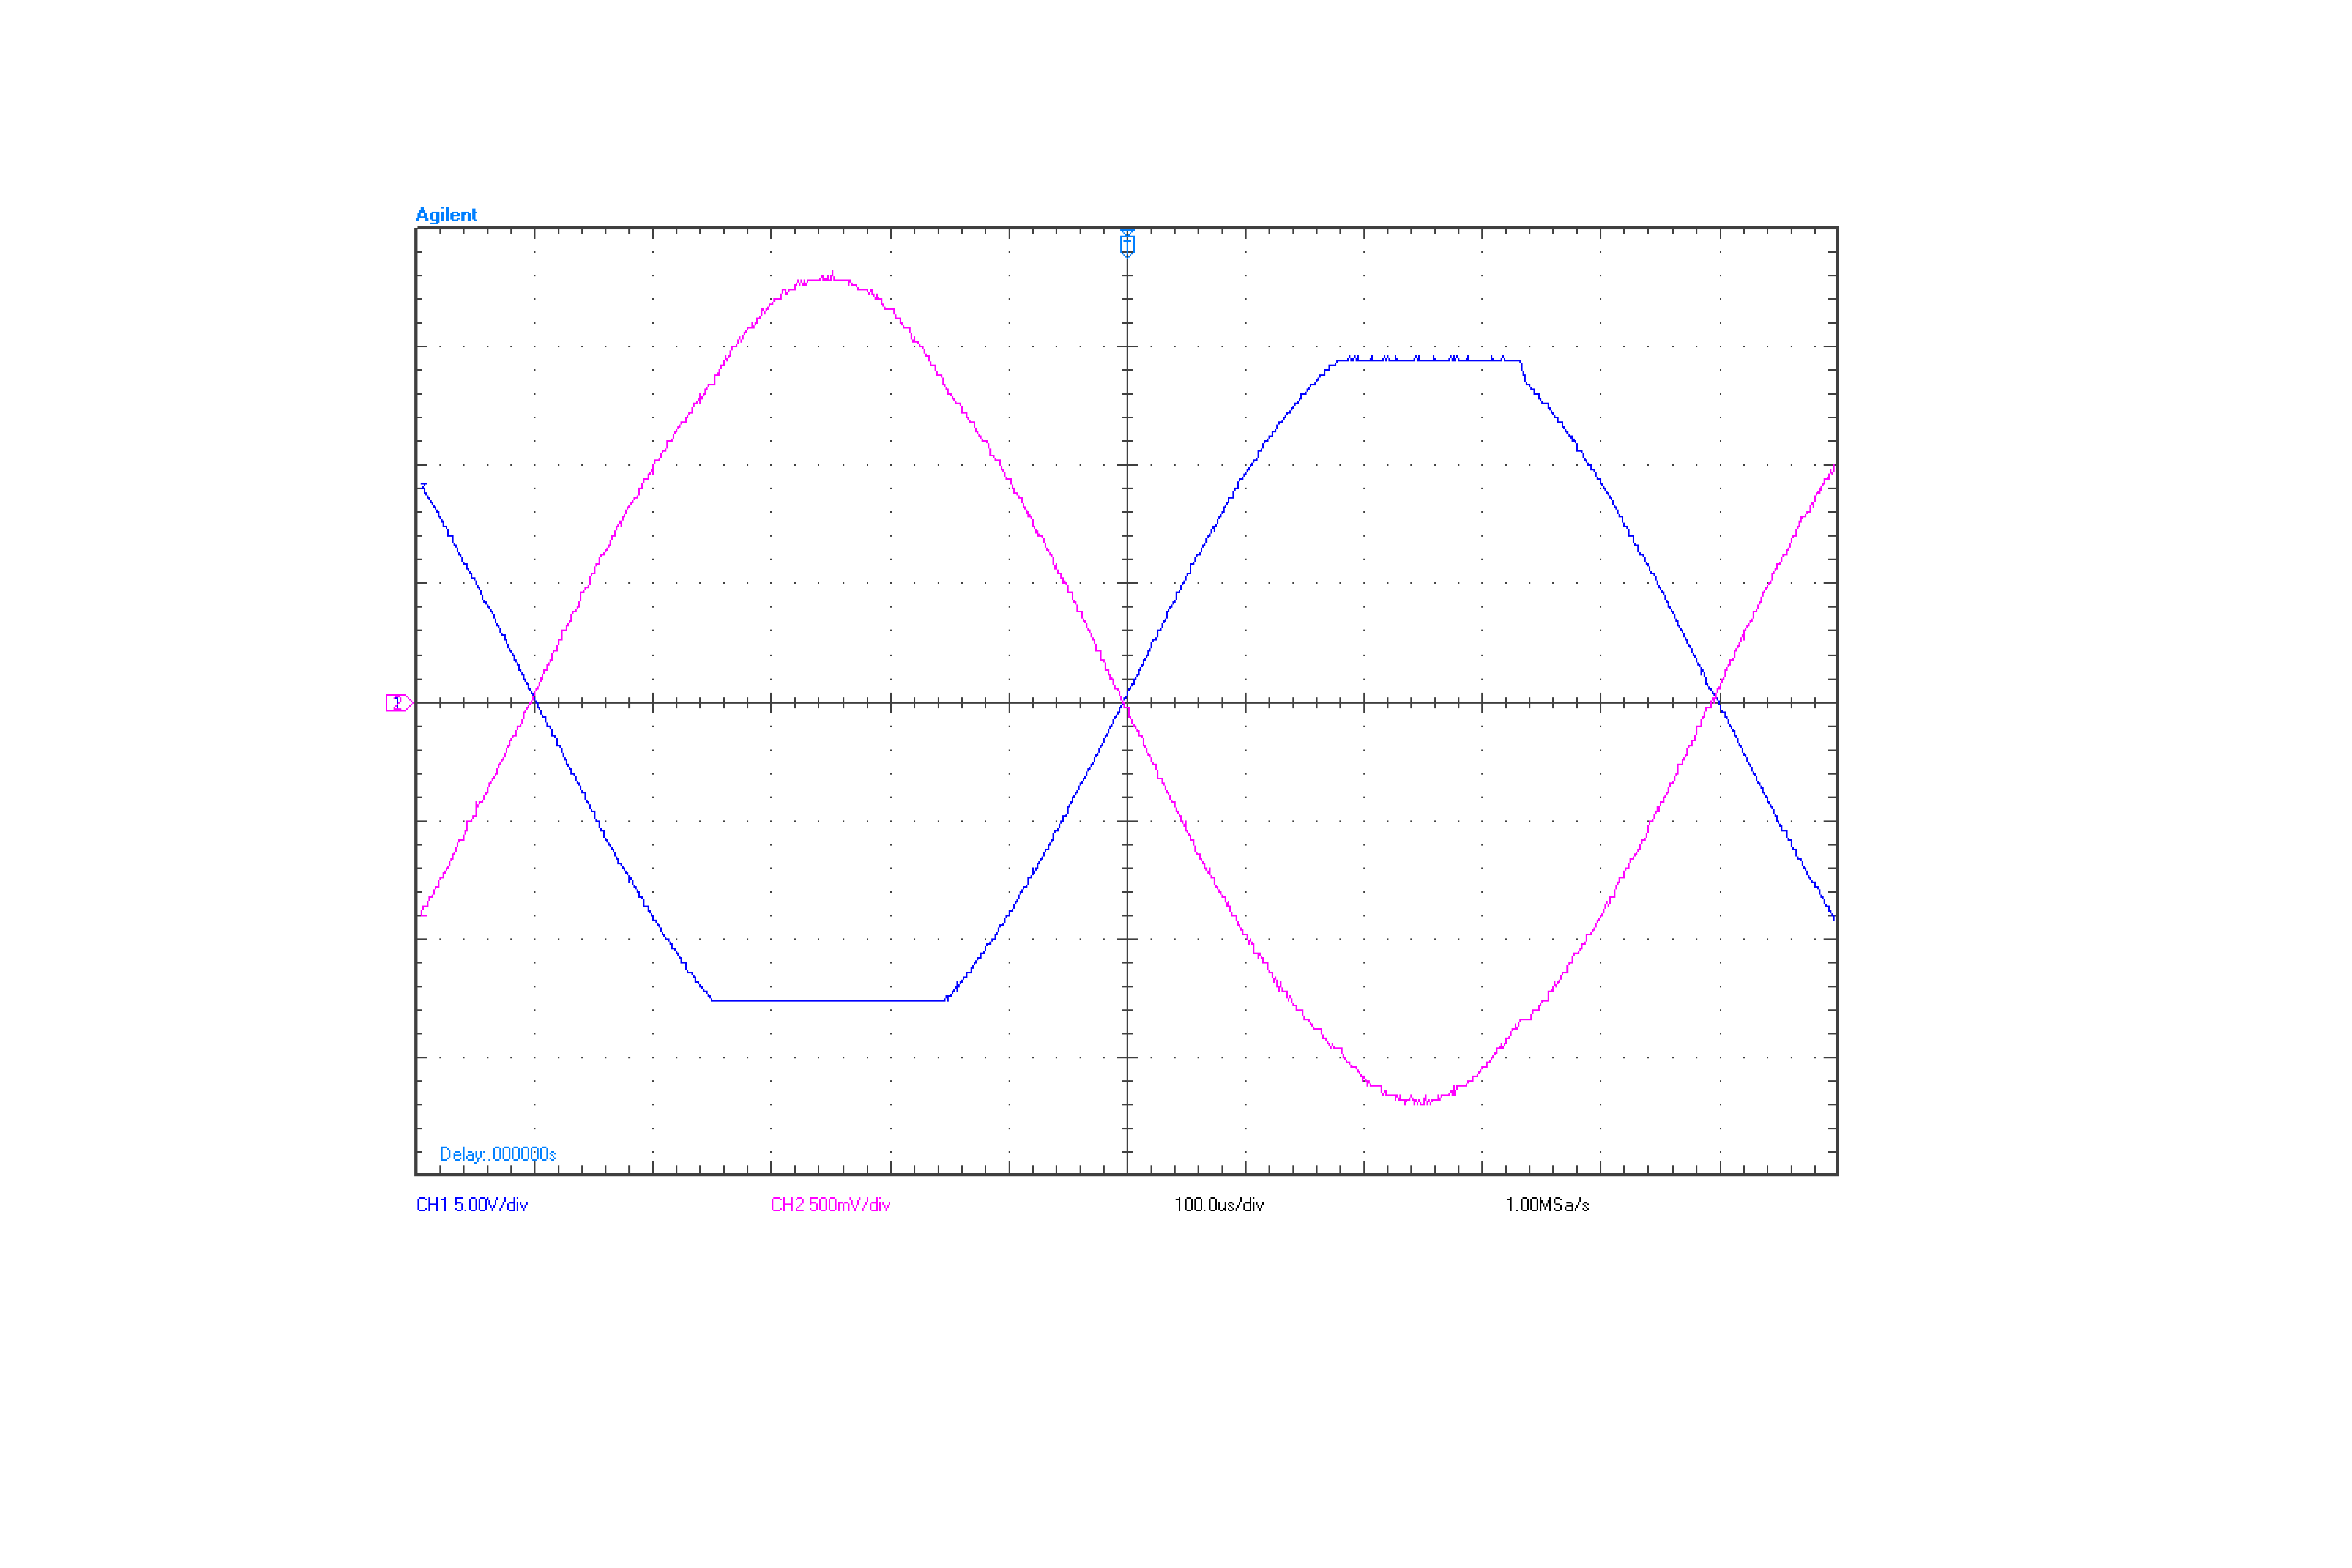
\includegraphics[height=70mm]{Result/Reverse/reverse-Hannten(input_1000mV_output_9120mV).png}
    \figcaption{歪みがすこし現れている波形}
    \label{fig:7-1-3}
\end{figure}
\begin{figure}[H]
    \centering
    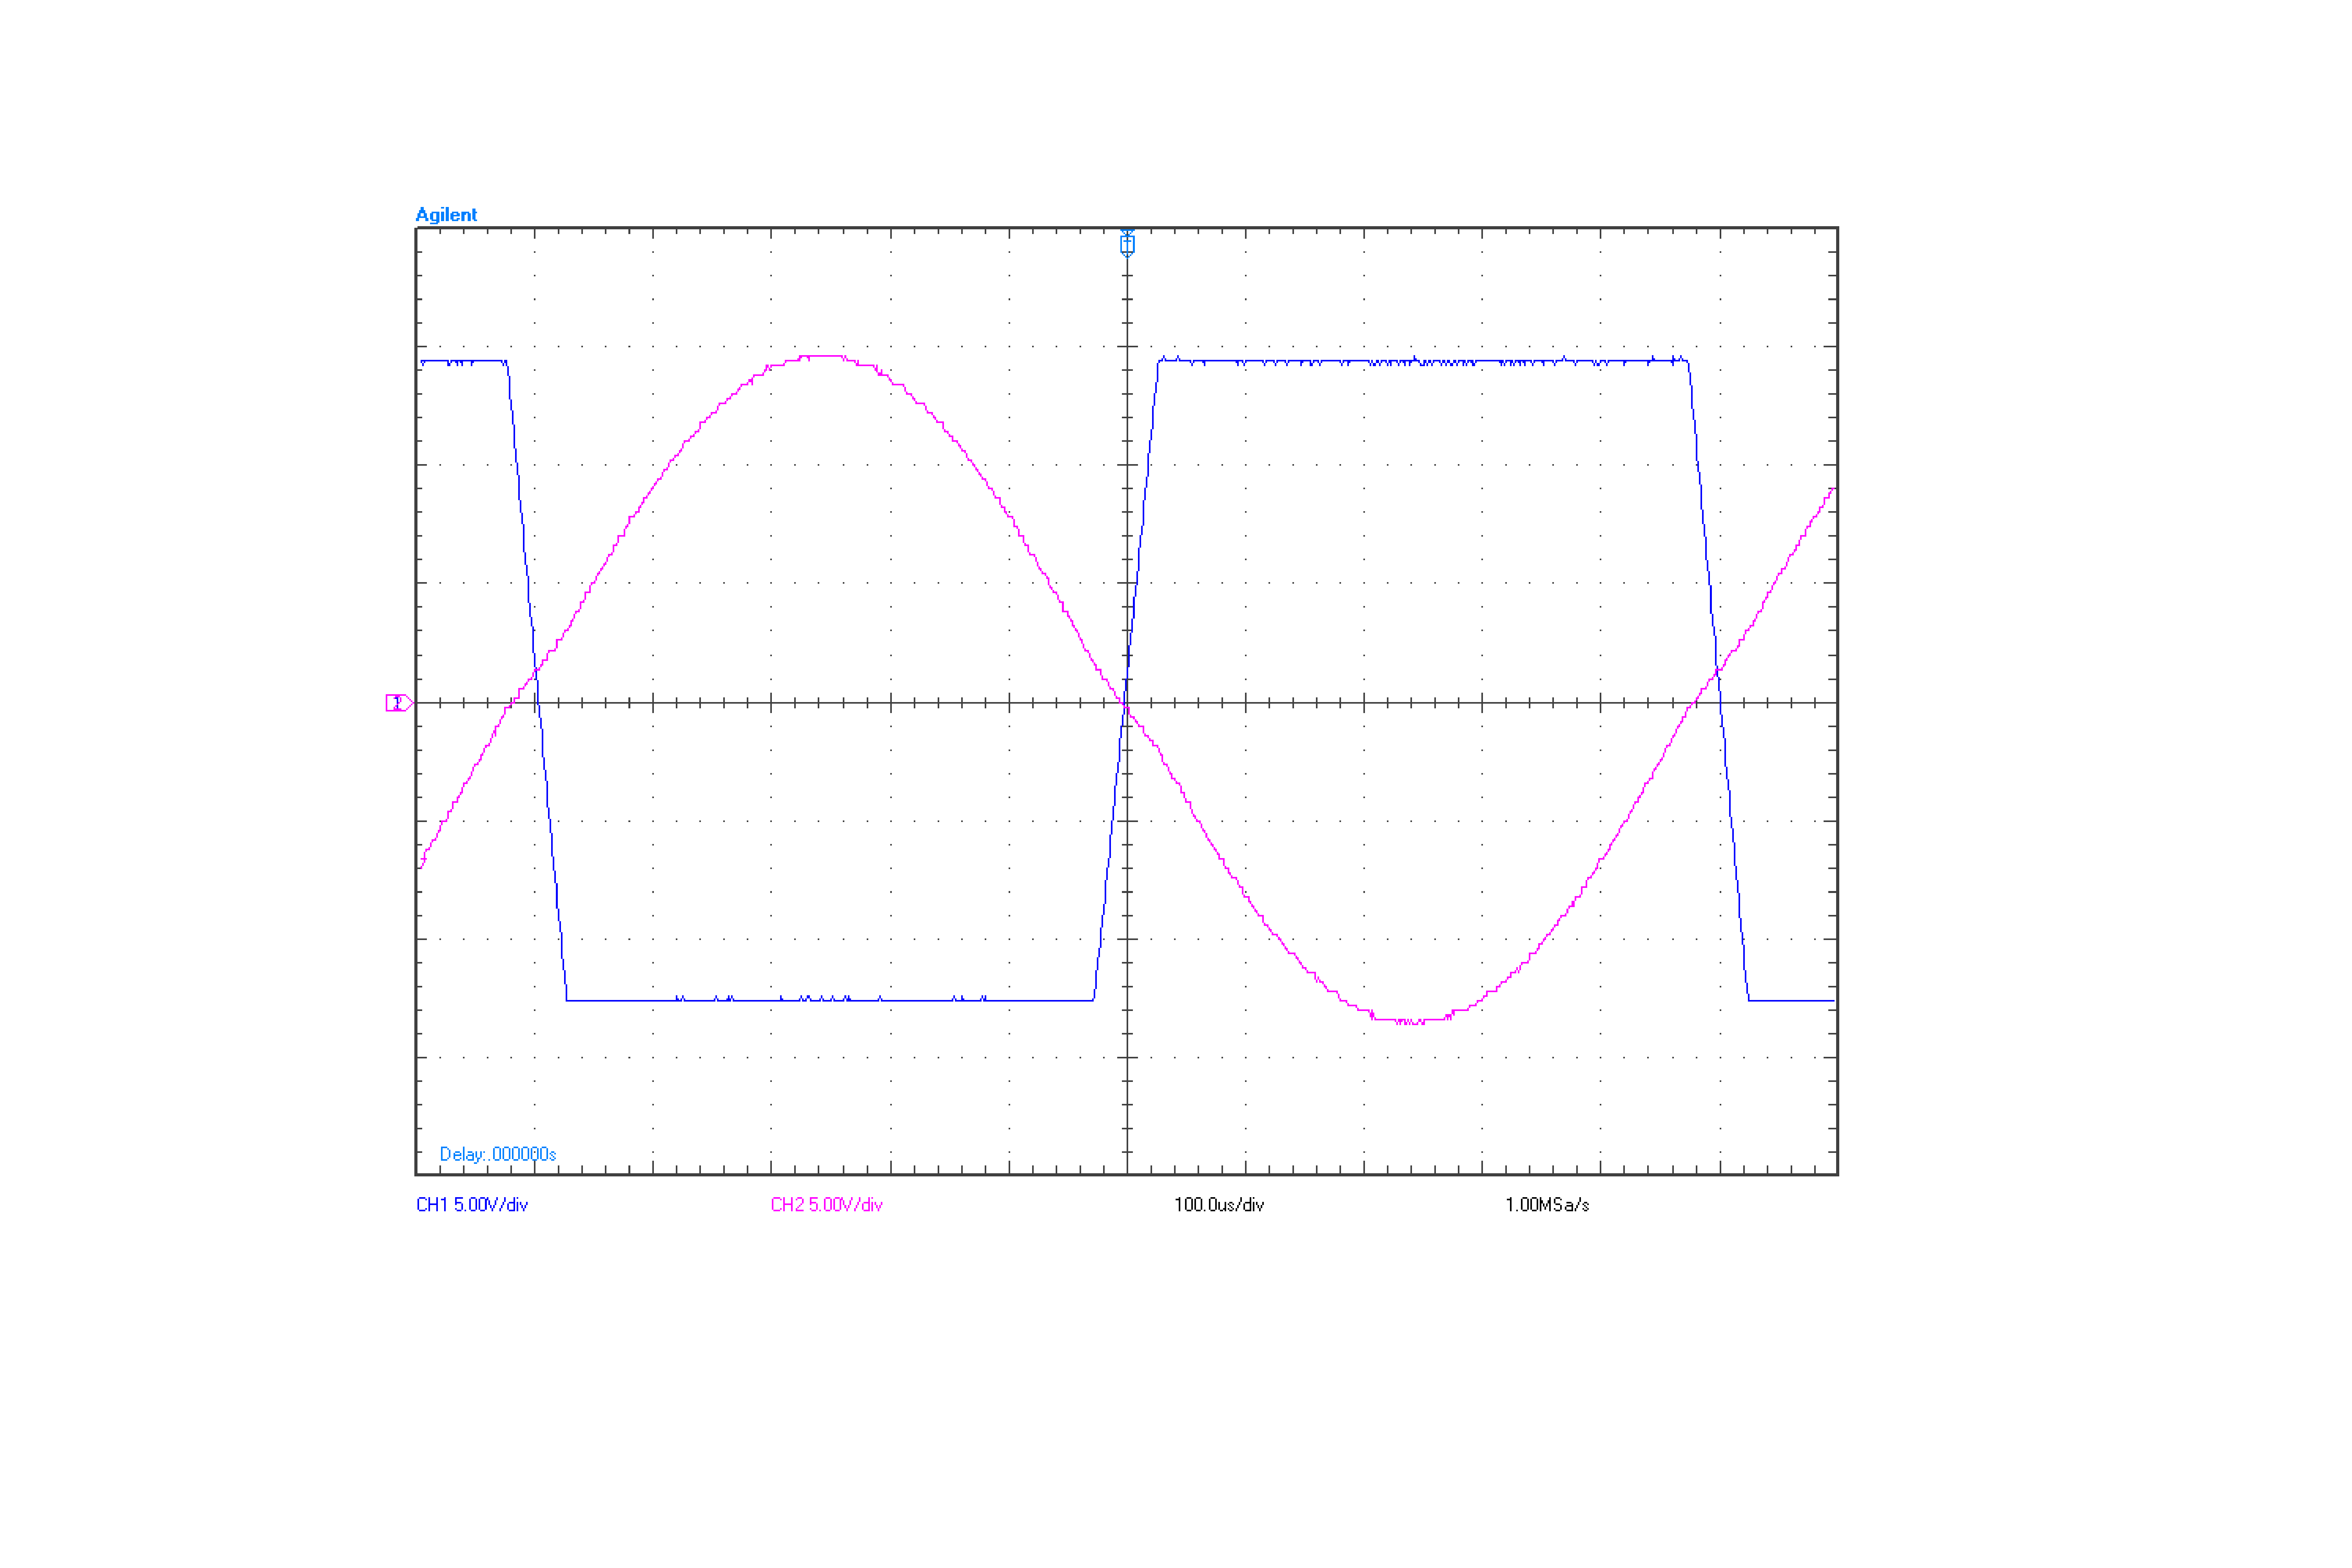
\includegraphics[height=70mm]{Result/Reverse/reverse-Hannten(input_8120mV_output_12200mV).png}
    \figcaption{歪みの顕著な波形}
    \label{fig:7-1-4}
\end{figure}


\newpage
\subsection{[減算増幅回路の特性測定結果の処理]}
5.2に示した実験について,以下の表\ref{tbl:7-2-1}に測定した値を,図\ref{fig:7-2-1}に測定値をもとにした伝達特性のグラフを示す.
\begin{figure}[H]
	\begin{tabular}{cc}
		\begin{minipage}{0.33\hsize}
			\normalsize
			\tblcaption{測定値}
			\label{tbl:7-2-1}
			\centering
			\small
			\begin{tabular}{|r|r|}\hline
                入力電圧 Vi  [V] & 出力電圧 Vo [V] \\\hline
                0.01 & 0.11 \\\hline
                0.10 & 1.08 \\\hline
                0.25 & 2.70 \\\hline
                0.50 & 5.41 \\\hline
                0.75 & 8.50 \\\hline
                1.00 & 9.60 \\\hline
                1.25 & 10.30 \\\hline
                1.50 & 10.80 \\\hline
                2.00 & 11.20 \\\hline
                2.50 & 11.60 \\\hline
                3.00 & 11.90 \\\hline
            \end{tabular}
			\normalsize
		\end{minipage}
		\begin{minipage}{0.66\hsize}
			\centering
			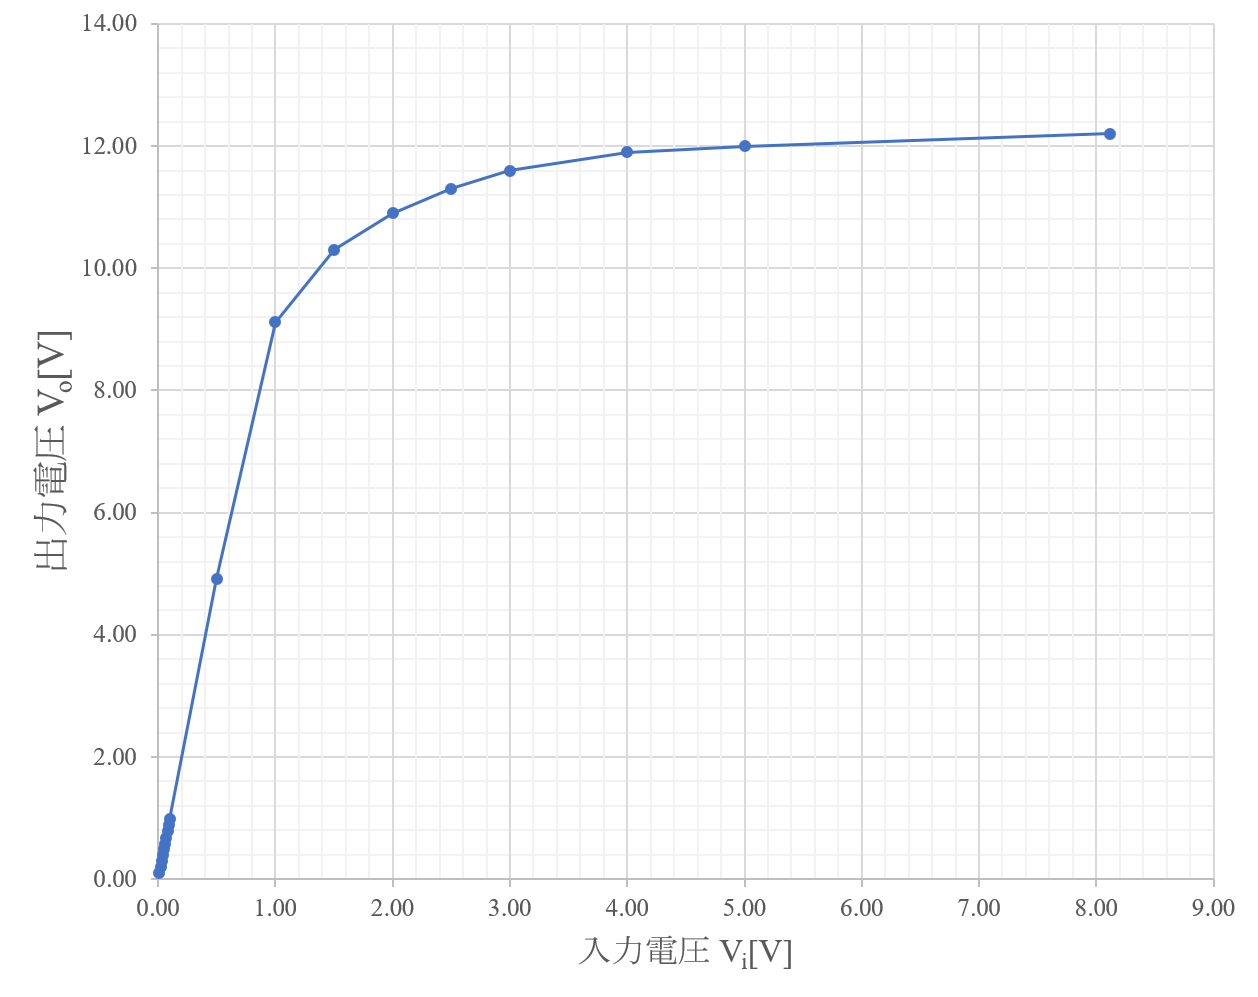
\includegraphics[width = 0.9\hsize]{experiment/7-2-1.png}
			\figcaption{制作した非反転増幅回路の伝達特性}
			\label{fig:7-2-1}
		\end{minipage}
	\end{tabular}
\end{figure}
また.以下にデジタルオシロスコープを用いて測定した歪み波形を示す.
\begin{figure}[H]
    \centering
    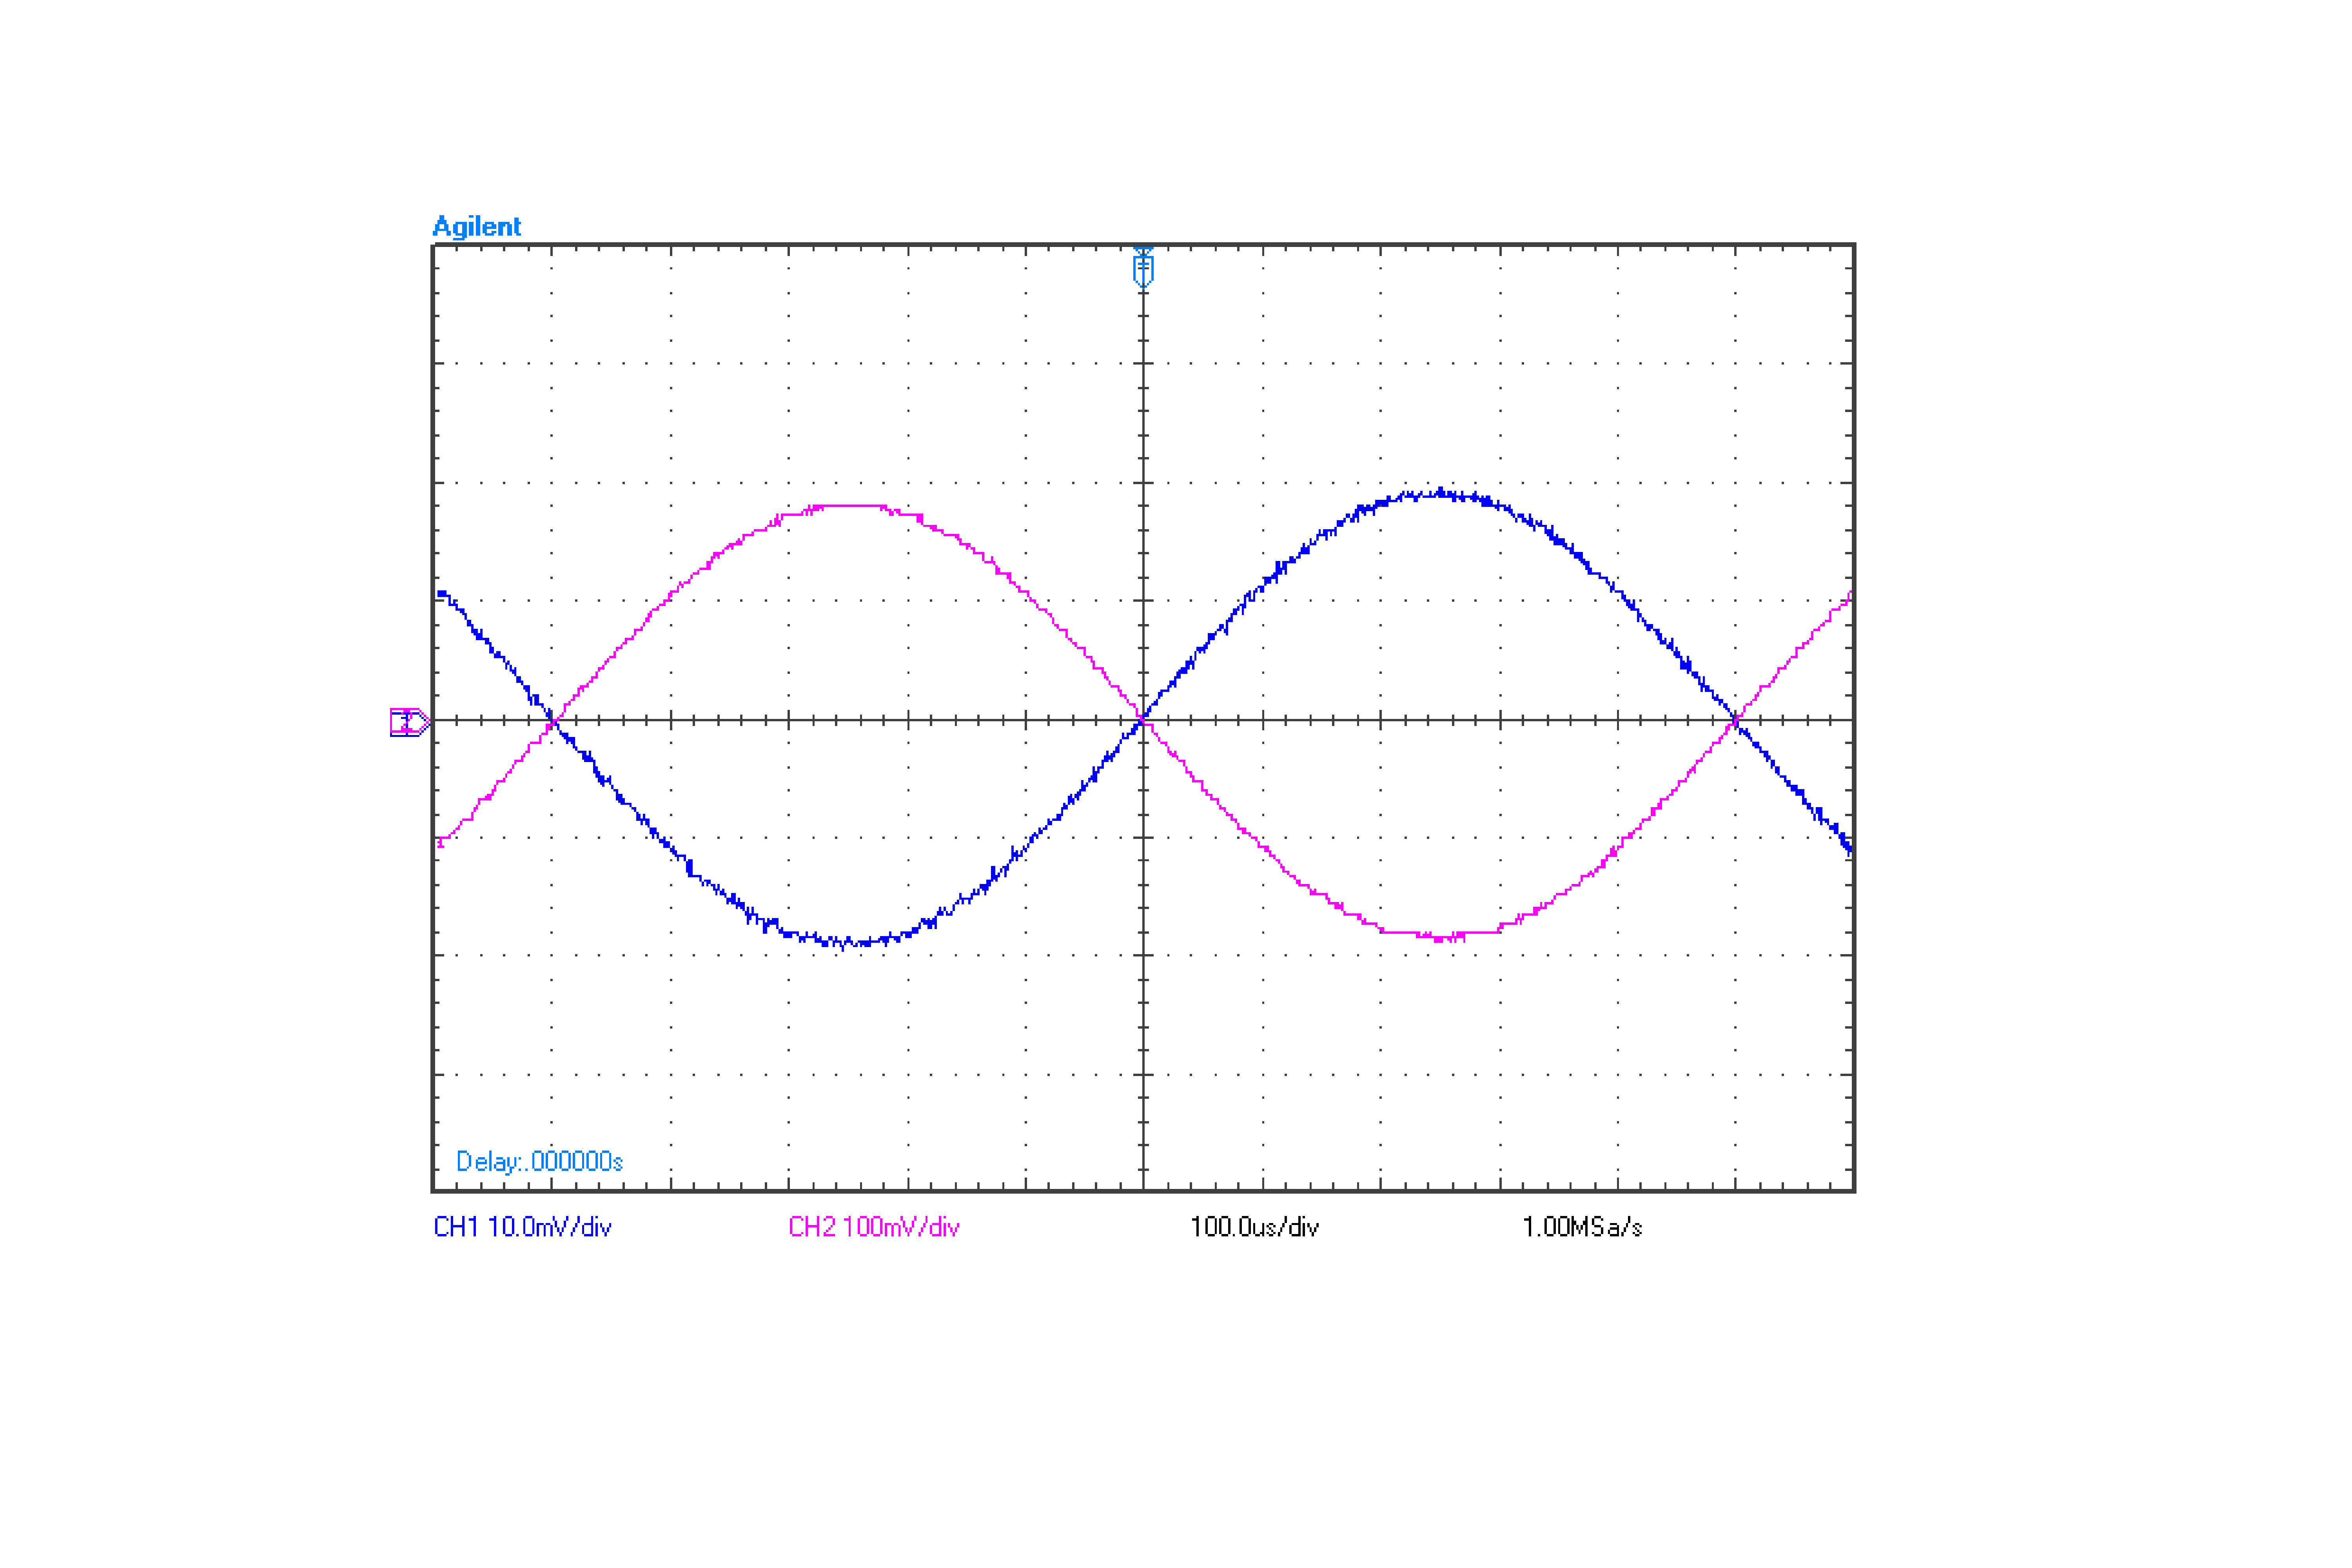
\includegraphics[height=70mm]{Result/Reverse/reverse-Hannten(input_10mV_output_95mV).png}
    \figcaption{歪みのない波形}
    \label{fig:7-2-2}
\end{figure}
\begin{figure}[H]
    \centering
    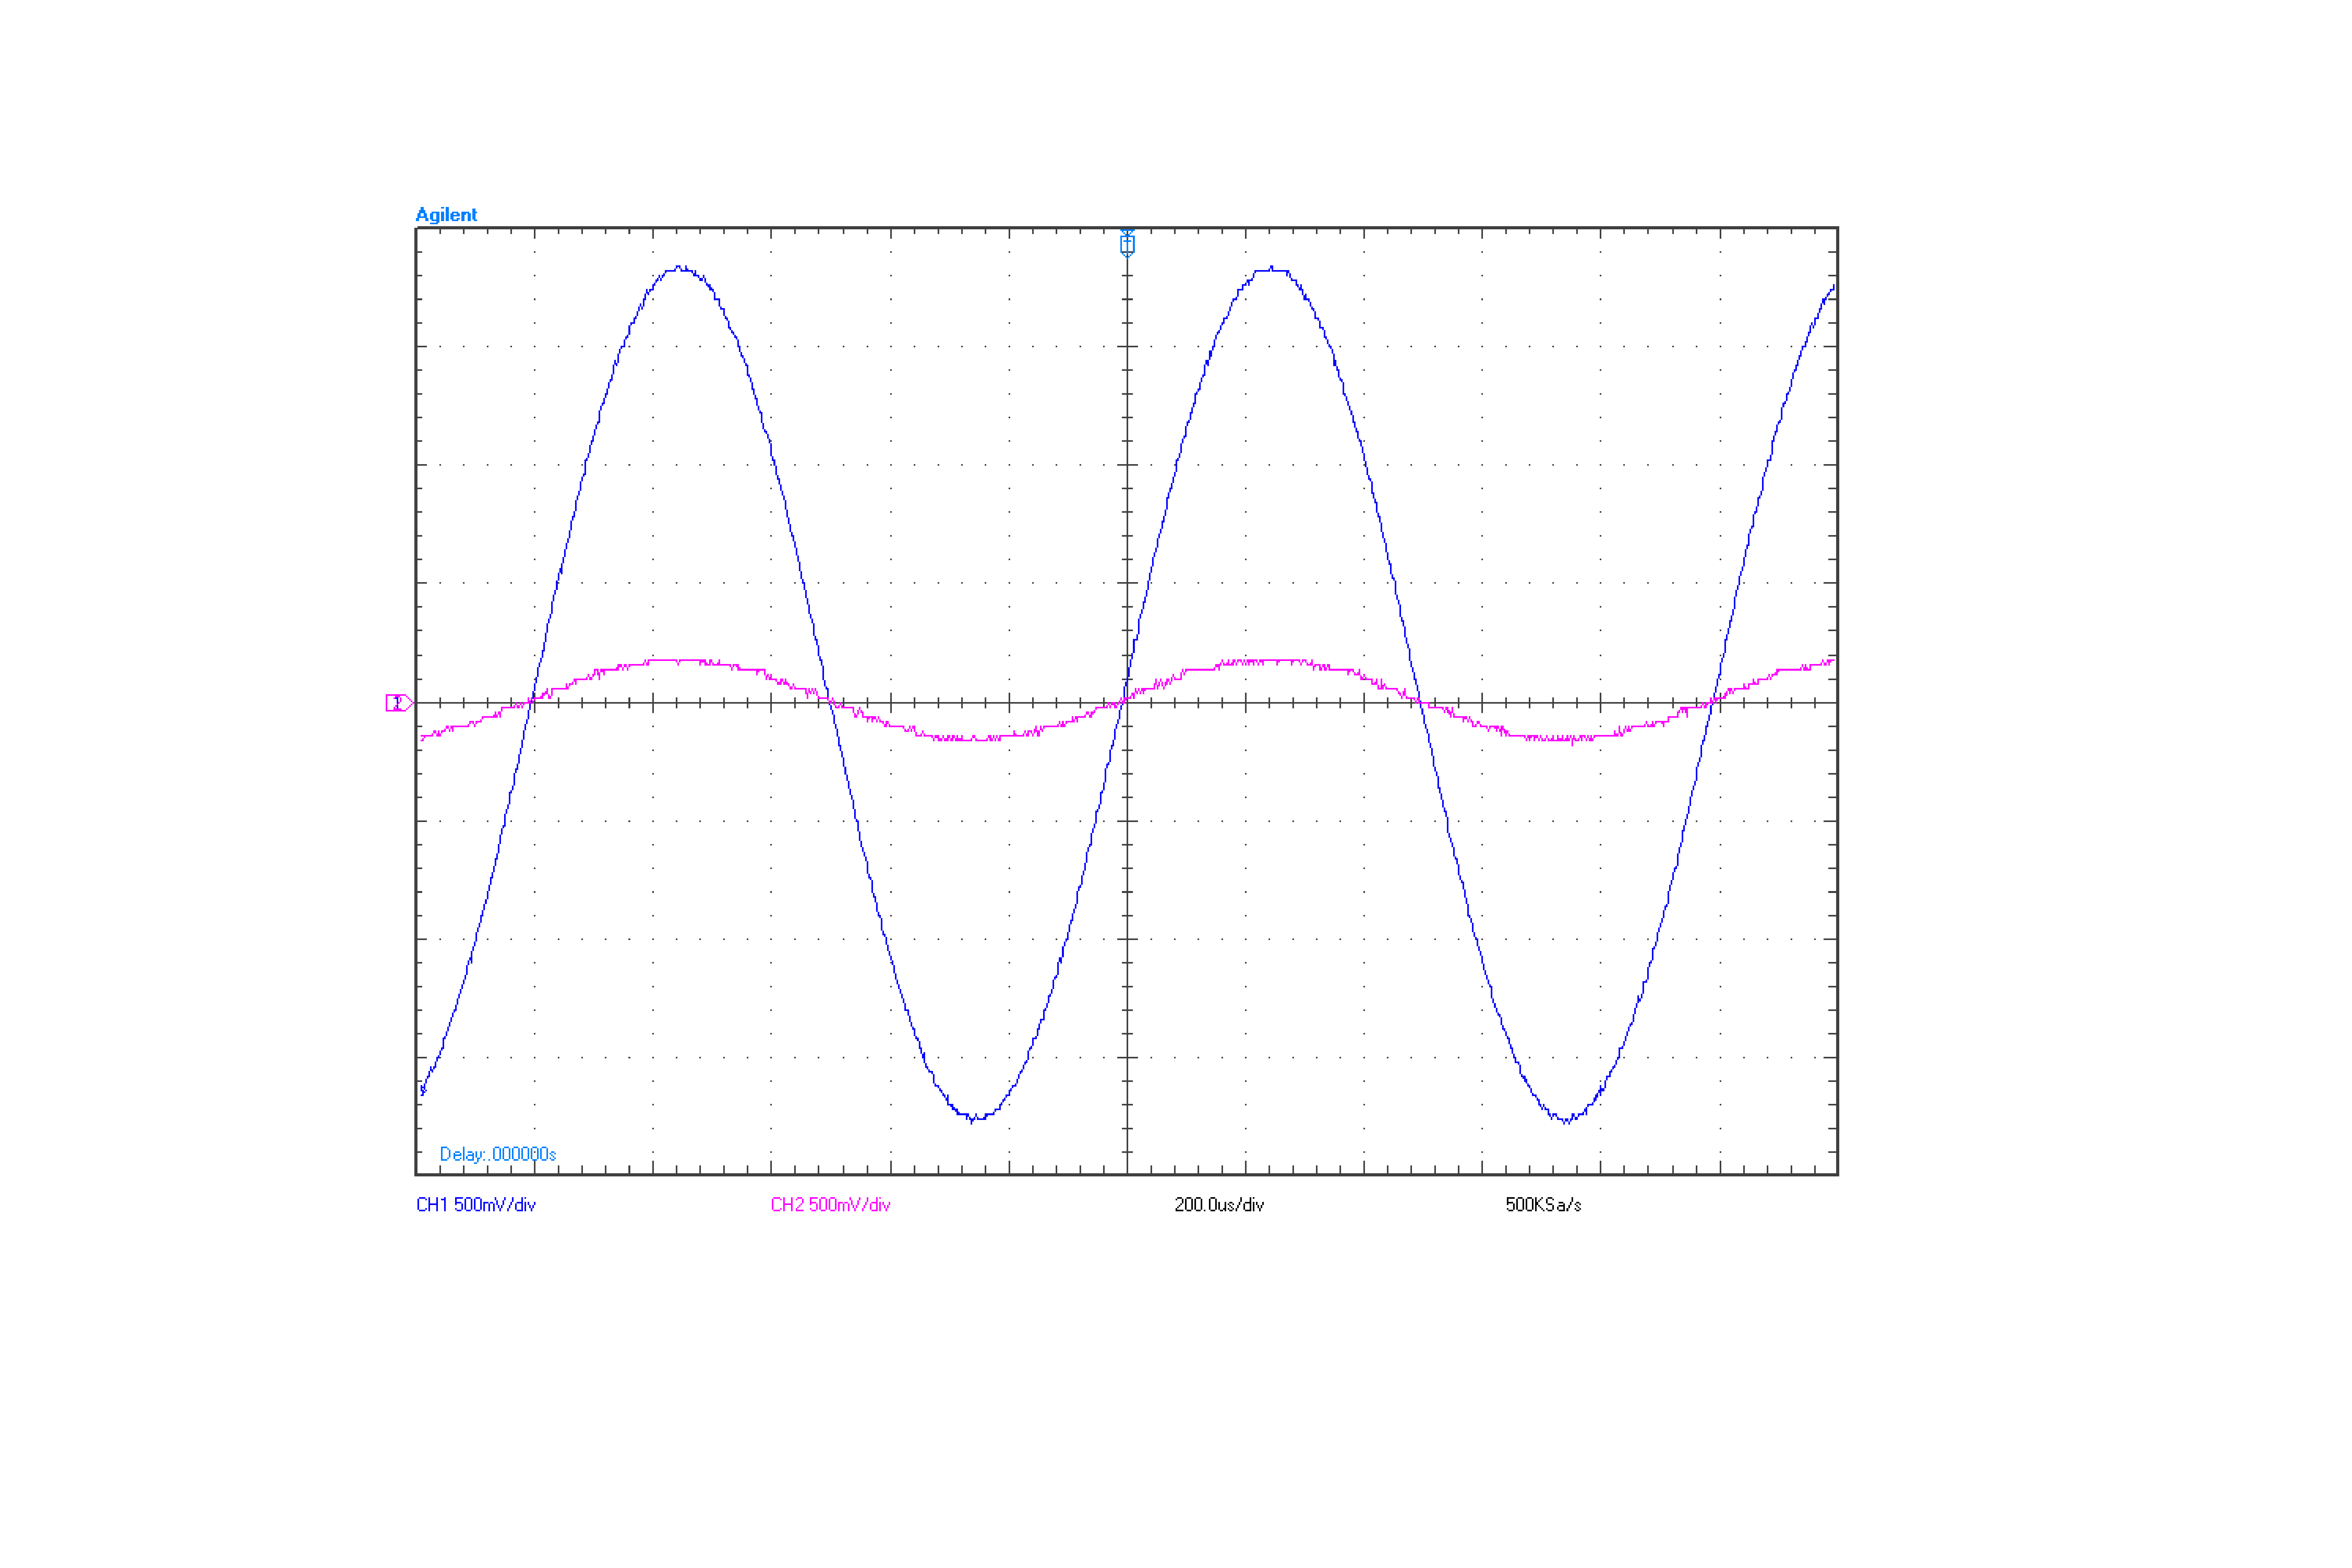
\includegraphics[height=70mm]{Result/Reverse/reverse-Hihannten(input_1000mV_output_9600mV).png}
    \figcaption{歪みがすこし現れている波形}
    \label{fig:7-2-3}
\end{figure}
\begin{figure}[H]
    \centering
    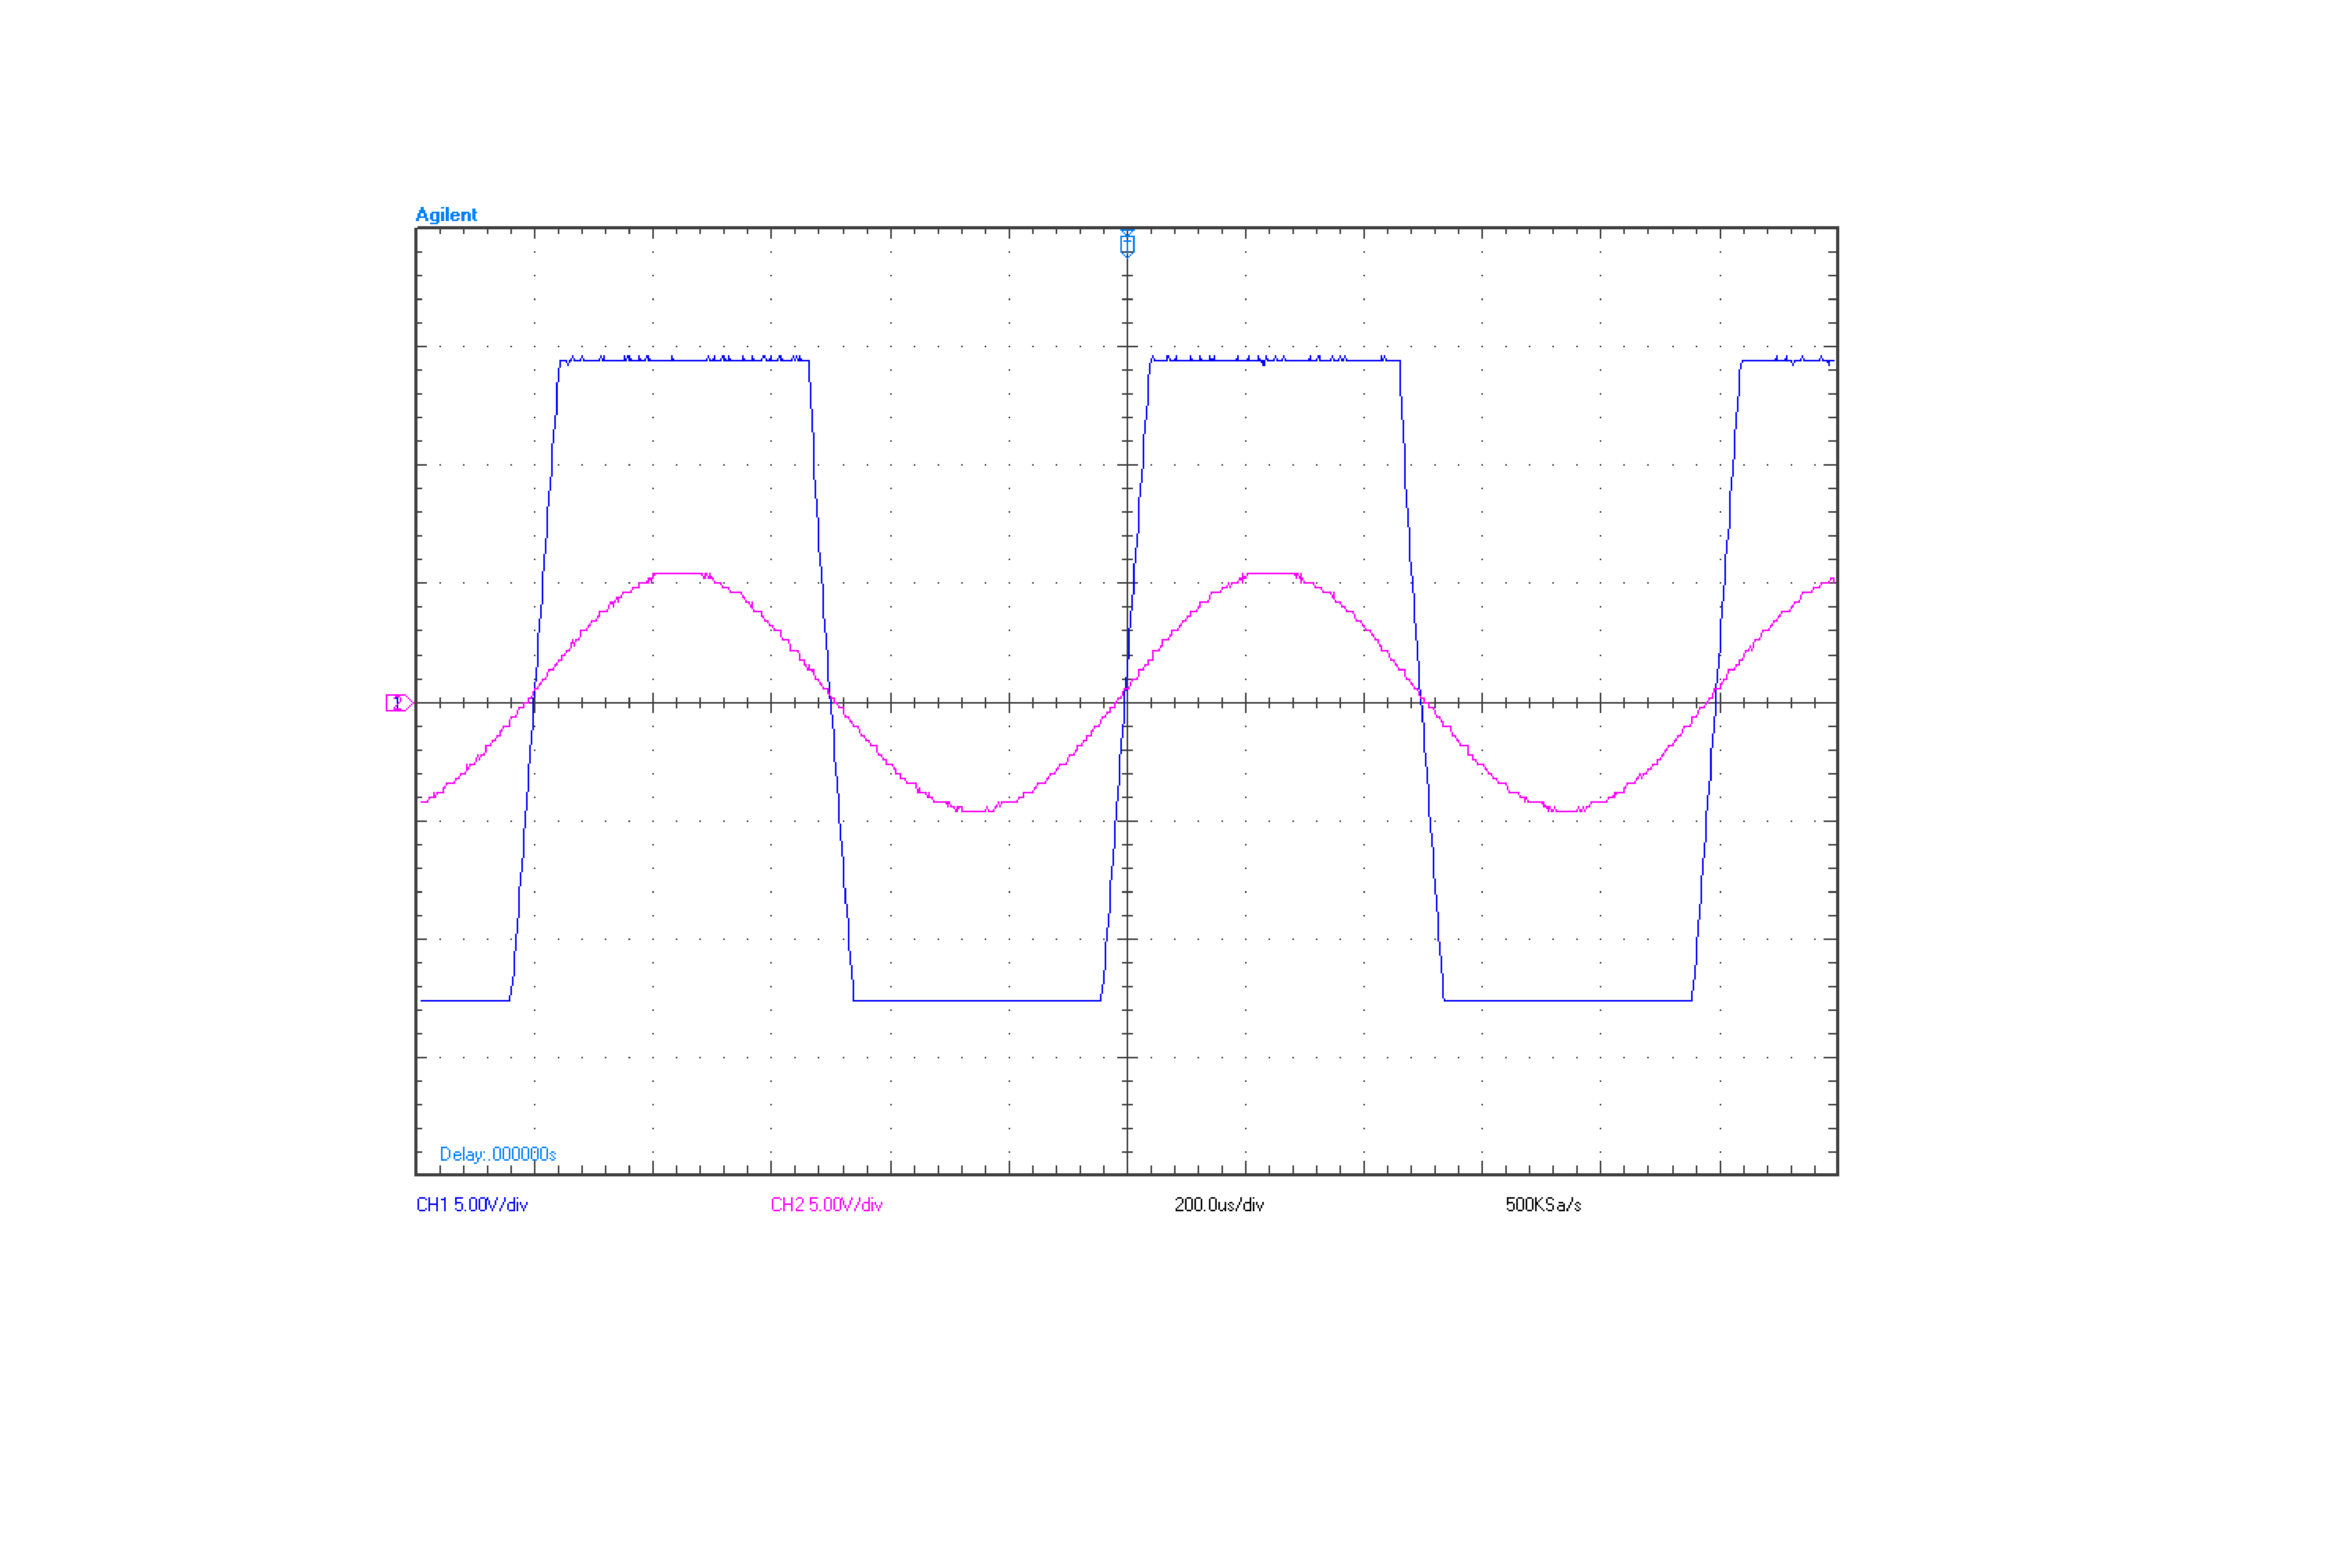
\includegraphics[height=70mm]{Result/Reverse/reverse-Hihannten(input_3000mV_output_11900mV).png}
    \figcaption{歪みの顕著な波形}
    \label{fig:7-2-4}
\end{figure}


\newpage
\subsection{[加算回路の特性測定結果の処理]}
5.3に示した実験について,以下の表\ref{tbl:7-3-1}に測定した値を,図\ref{fig:7-3-1}に測定結果をもとに作成した入出力の関係のグラフを示す.
また,このとき,一方の入力電圧$V_2$は$0.33[V]$に固定して実験を行った.
\begin{figure}[H]
	\begin{tabular}{cc}
		\begin{minipage}{0.33\hsize}
			\normalsize
			\tblcaption{測定値}
			\label{tbl:7-3-1}
			\centering
			\small
			\begin{tabular}{|r|r|}\hline
                入力電圧 V1  [V] & 出力電圧 Vo [V] \\\hline
                0.002 & 3.3 \\\hline
                0.101 & 4.37 \\\hline
                0.207 & 5.43 \\\hline
                0.307 & 6.45 \\\hline
                0.402 & 7.42 \\\hline
                0.505 & 8.45 \\\hline
                0.602 & 9.44 \\\hline
                0.705 & 10.47 \\\hline
                0.804 & 11.47 \\\hline
                0.904 & 12.47 \\\hline
                1.008 & 12.86 \\\hline
                1.107 & 12.88 \\\hline
                1.207 & 12.89 \\\hline
            \end{tabular}
			\normalsize
		\end{minipage}
		\begin{minipage}{0.66\hsize}
			\centering
			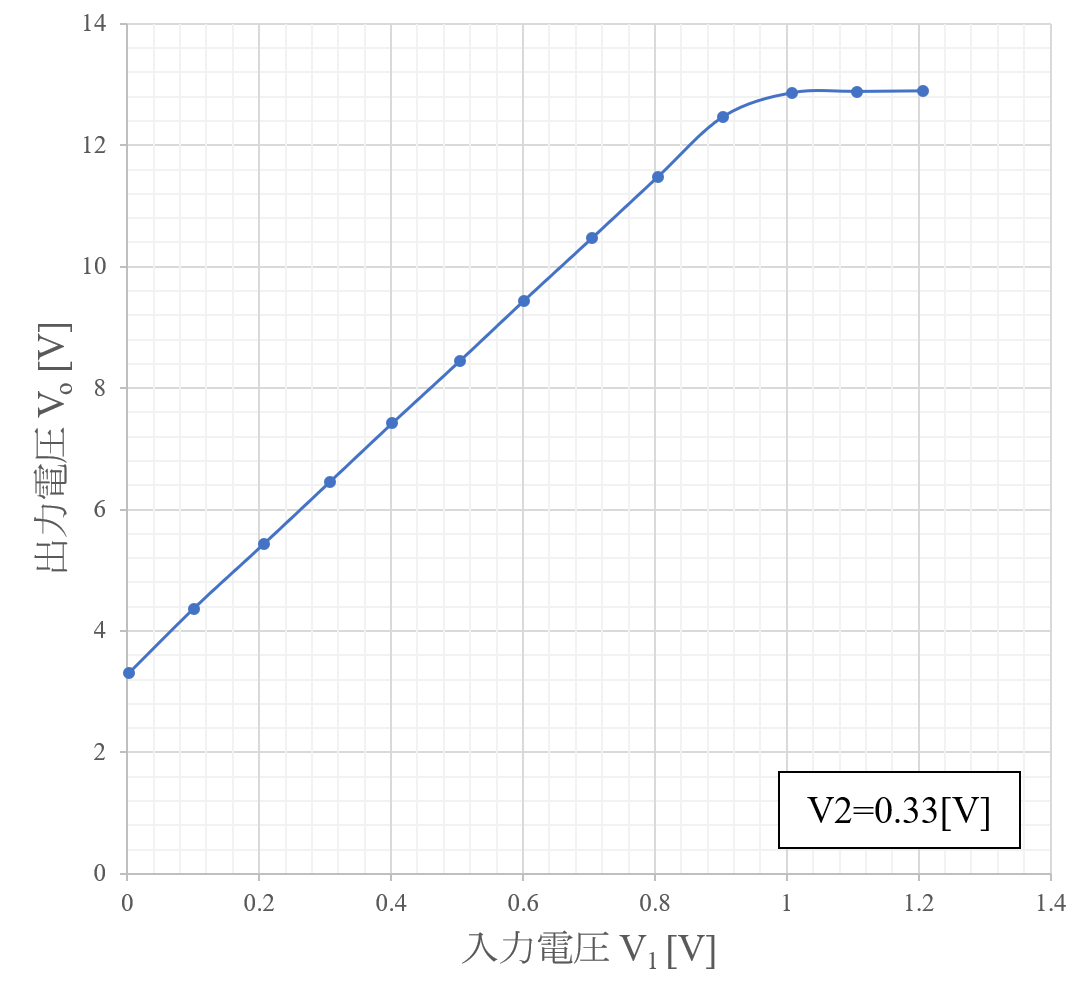
\includegraphics[width = 0.7\hsize]{experiment/7-3-1.png}
			\figcaption{加算回路の入出力の関係}
			\label{fig:7-3-1}
		\end{minipage}
	\end{tabular}
\end{figure}


\newpage
\subsection{[減算回路の特性測定結果の処理]}
5.4に示した実験について,以下の表\ref{tbl:7-4-1}に測定した値を,図\ref{fig:7-4-1}に測定結果をもとに作成した入出力の関係のグラフを示す.
また,このとき,一方の入力電圧$V_2$は$1.502[V]$に固定して実験を行った. 
\begin{figure}[H]
	\begin{tabular}{cc}
		\begin{minipage}{0.33\hsize}
			\normalsize
			\tblcaption{測定値}
			\label{tbl:7-4-1}
			\centering
			\small
			\begin{tabular}{|r|r|}\hline
                入力電圧 V1  [V] & 出力電圧 Vo [V] \\\hline
                0.002 & 3.3 \\\hline
                0.101 & 4.37 \\\hline
                0.207 & 5.43 \\\hline
                0.307 & 6.45 \\\hline
                0.402 & 7.42 \\\hline
                0.505 & 8.45 \\\hline
                0.602 & 9.44 \\\hline
                0.705 & 10.47 \\\hline
                0.804 & 11.47 \\\hline
                0.904 & 12.47 \\\hline
                1.008 & 12.86 \\\hline
                1.107 & 12.88 \\\hline
                1.207 & 12.89 \\\hline
            \end{tabular}
			\normalsize
		\end{minipage}
		\begin{minipage}{0.66\hsize}
			\centering
			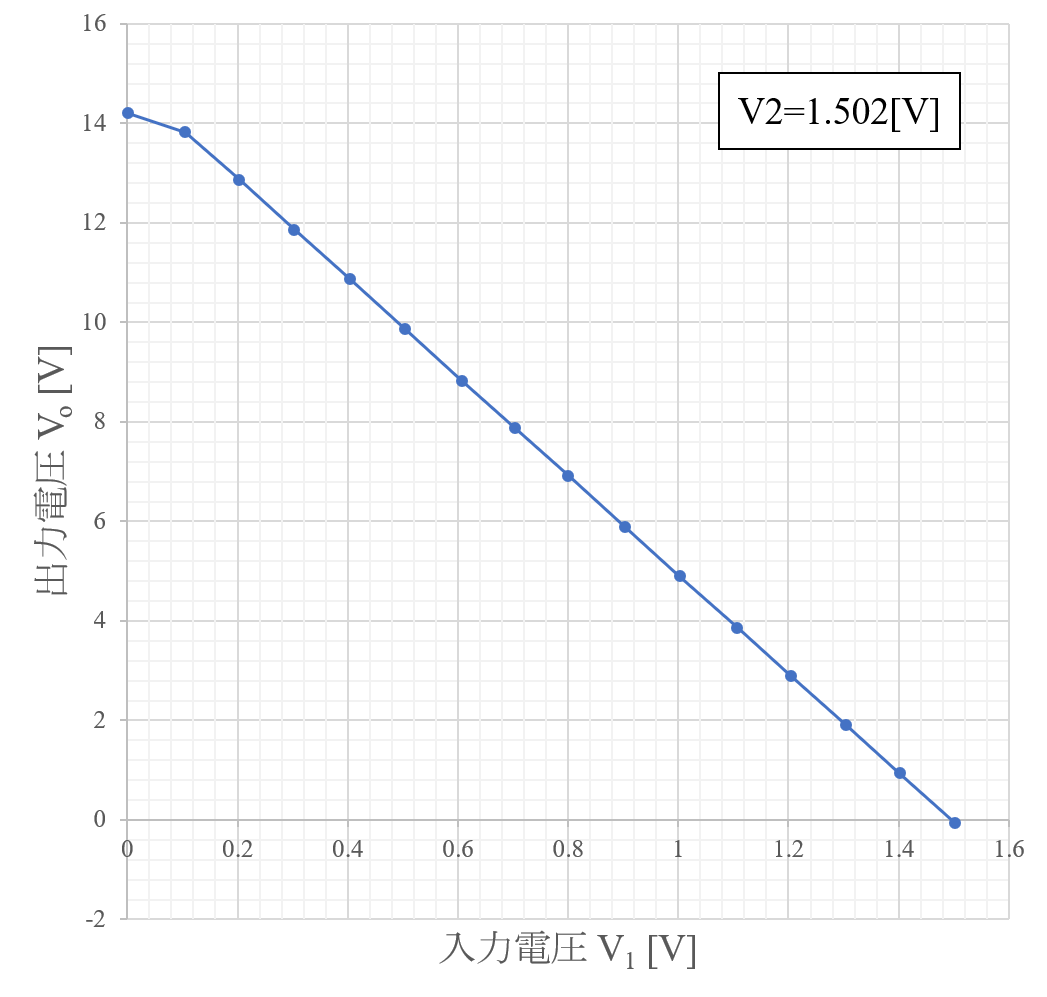
\includegraphics[width = 0.7\hsize]{experiment/7-4-1.png}
			\figcaption{加算回路の入出力の関係}
			\label{fig:7-4-1}
		\end{minipage}
	\end{tabular}
\end{figure}

\newpage
\subsection{応用回路の測定結果の処理}
6.に示した実験の測定結果を以下図\ref{fig:7-5-1}~\ref{fig:7-5-2}に示す.
\begin{figure}[H]
    \centering
    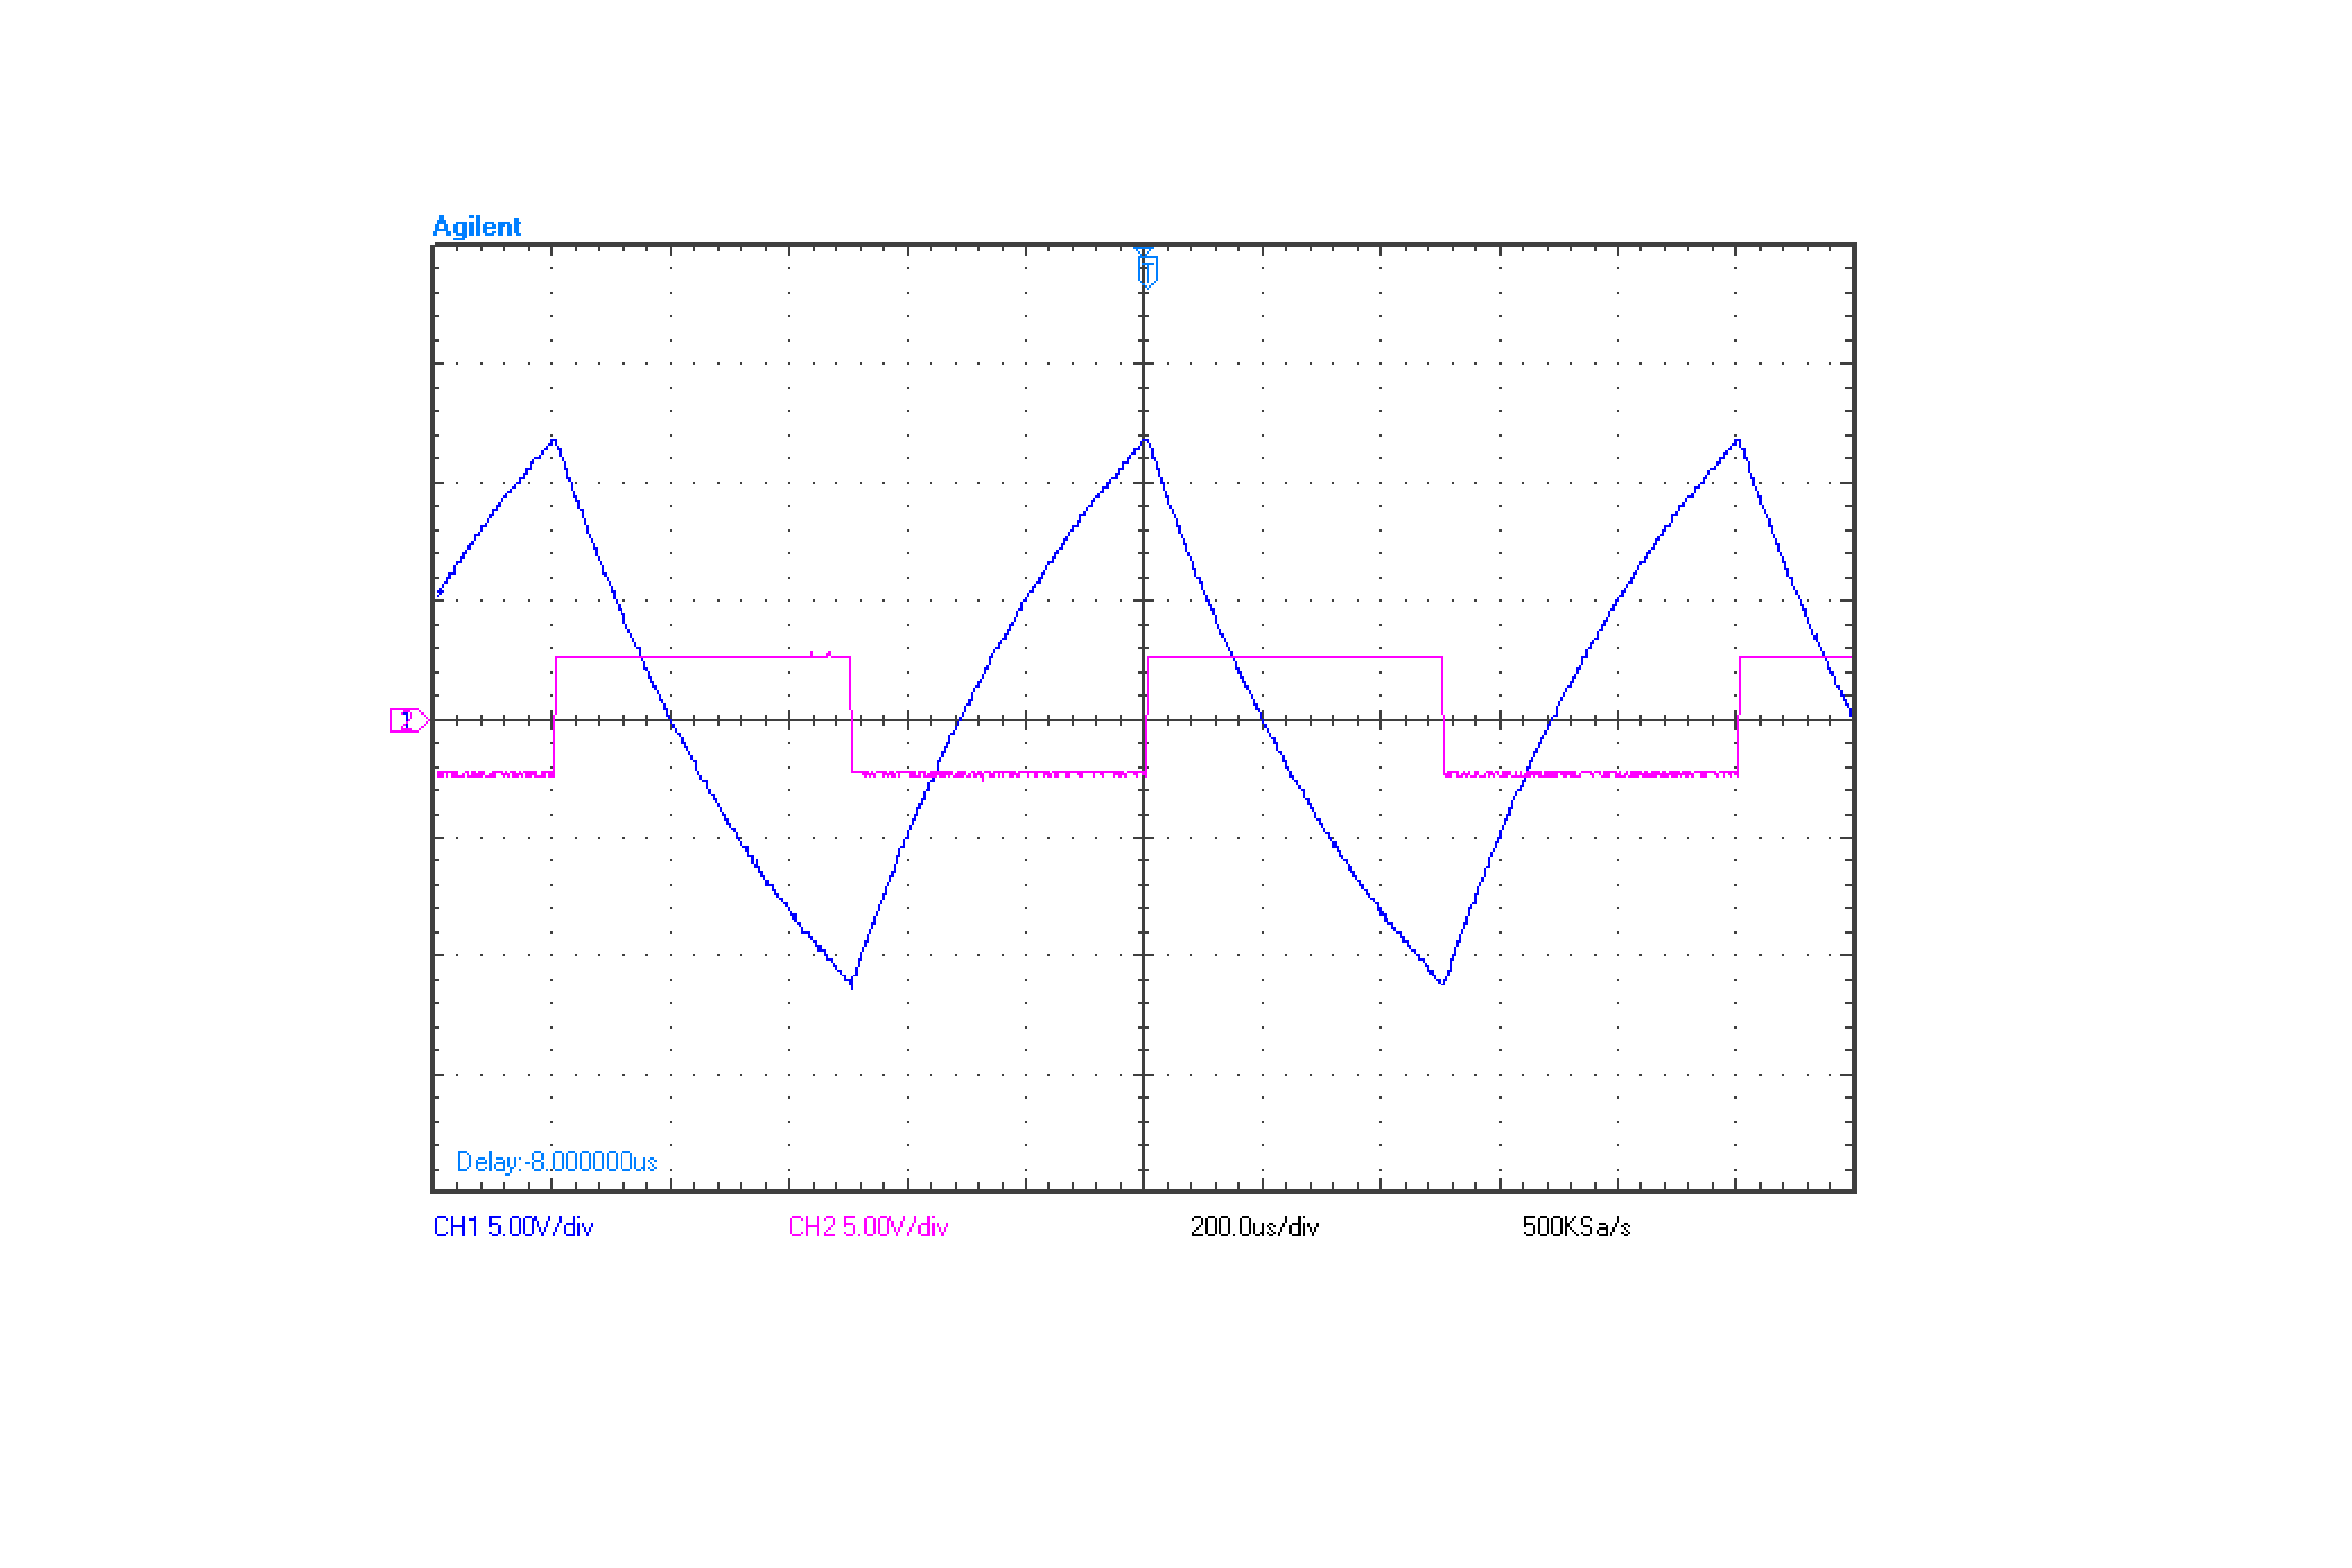
\includegraphics[height=70mm]{Result/Reverse/reverse-1kHz_4900pF.png}
    \figcaption{コンデンサを4900pFとしたときの出力波形}
    \label{fig:7-5-1}
\end{figure}
\begin{figure}[H]
    \centering
    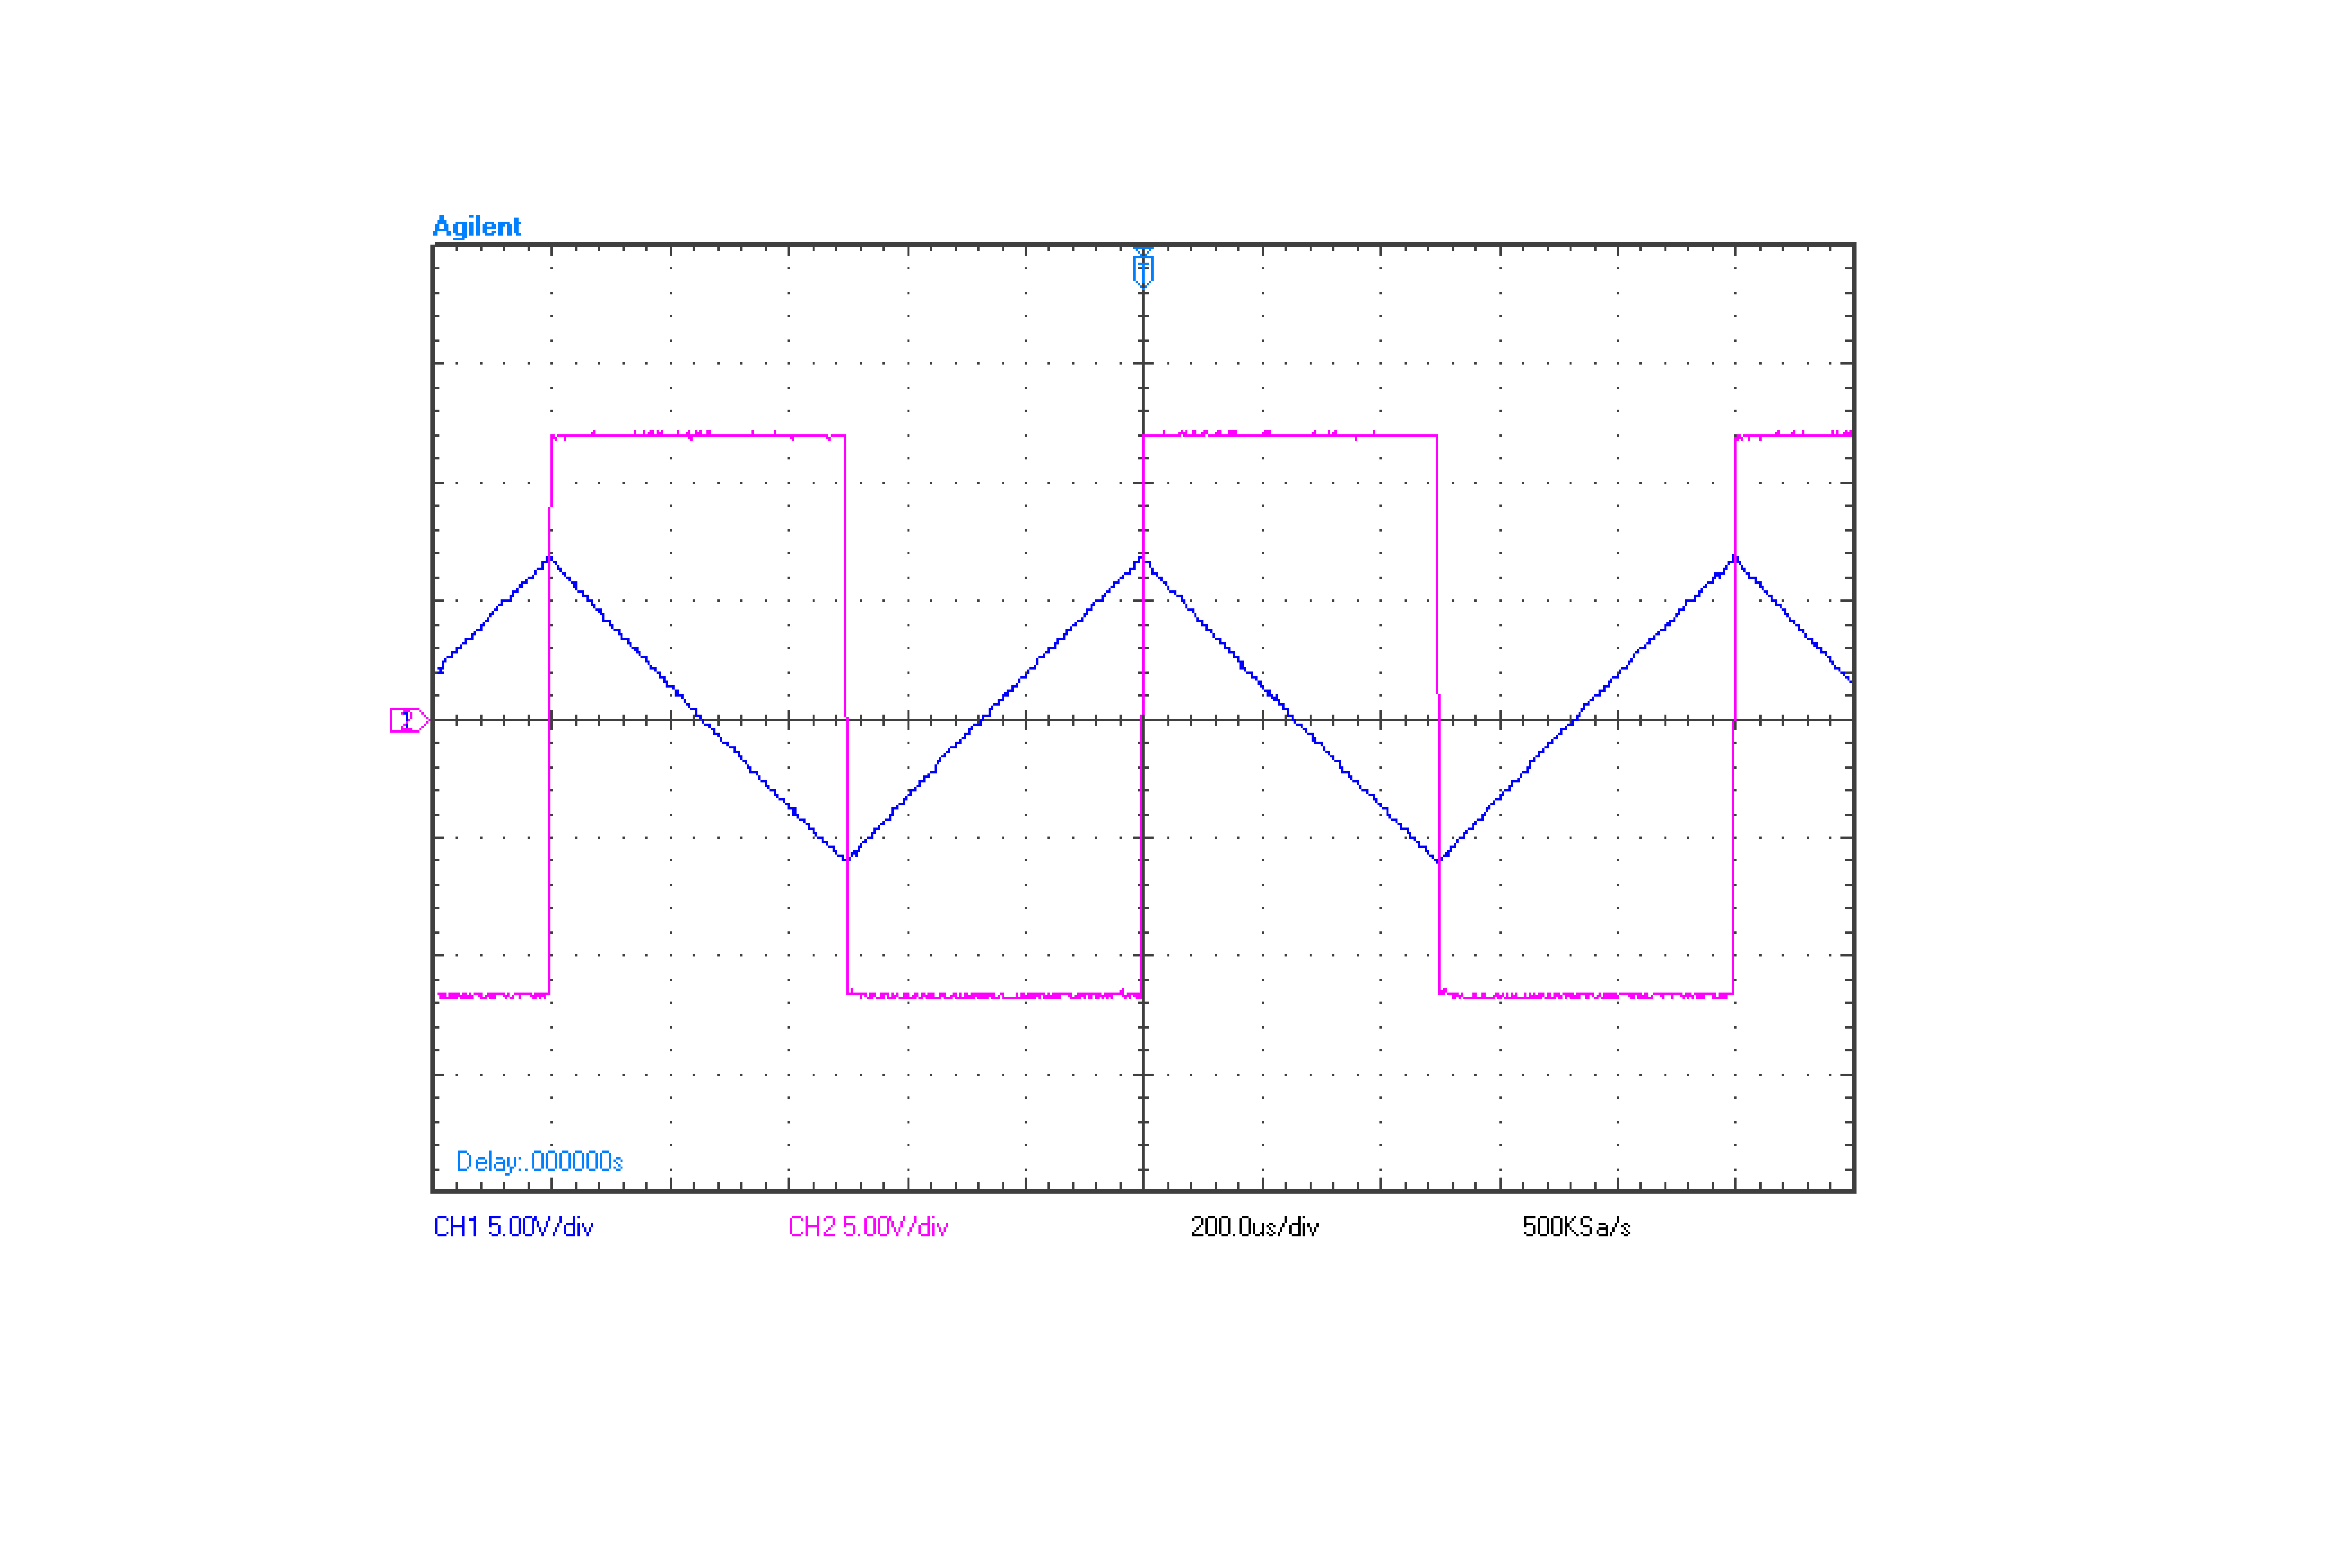
\includegraphics[height=70mm]{Result/Reverse/reverse-1kHz_47000pF.png}
    \figcaption{コンデンサを47000pFとしたときの出力波形}
    \label{fig:7-5-2}
\end{figure}


\newpage
\section{検討事項}
\begin{enumerate}
    \item デジタルボルトメーターにより入力電圧及び出力電圧を測定し,出力電圧が飽和すると測定誤差が大きくなる.なぜ測定誤差が大きくなるか,また この誤差を少なくするにはどうすればよいか考察せよ.\\
    
    出力電圧が飽和する,という状態は噛み砕いて表現すると「本来であればより大きな電圧が印加されているはずだが,IC等の定格によってある一定の数値以上の電圧は印加されなくなっている」状態と言える.つまり,前に示した図\ref{fig:7-2-4}のような歪みが生じているということである.

    \item 今回の実験は.,交流特性を測定したが,直流を入力信号として供給すれば,演算増幅器の直流特性が測定できる.それぞれの測定はどのような意味を持つか吟味せよ.\\

    \item 6の(2)の実験で得られた入出力波形の関係を周波数スペクトル解析しなさい. \\

\end{enumerate}



\end{document}